% !TEX root =paper.tex

\section{Reduction and payment}\label{sec:payment}

%FILL IN
%Since the reduction rule described in step 2 of the O-join construction depends only on whether an edge's top cuts are even, these reductions may result in cuts lower down in the hierarchy that are no longer  satisfied in the T-join solution. To fix this, we will ensure that for each near-mincut $S$, if the cut is odd, and  there are edges  $\delta ^\uparrow (S)$ that were reduced, then an equal amount of increase will be done on edges $f \in \delta ^\rightarrow (S)$.
%Our goal will be to show that the resulting expected increase in  $y_e$ for any edge $e$ is smaller than its expected decrease  due to its own reduction events.  Crucial to this will be to determine the probability that the cut $\delta (S)$ is odd given that an edge $f \in \delta ^\uparrow (S)$ is reduced.

In this section we prove \cref{thm:payment-main}. %Through this section we will refer to a \textit{slack vector} $s: E \to \R$, a \textit{decrease vector} $R: E \to \R$, and an \textit{increase vector} $I: E \to \R$. For any $F \subseteq E$, let $s(F) = \sum_{f \in F} s_f$, and similarly for $R,I$. 


%For the rest of the section we will work with edge bundles instead of individual edges.


% !TEX root =paper.tex


%In this section we show that there is a randomized matching procedure over our laminar family $\mathcal{L}$ such that all good edge bundles $e$ have $\E{y_e}$ strictly less than $x_e/4$. %Recall that edge bundles only contain edges from the $x$ component of $z^*$.

%In the following, as in previous sections, we will \textbf{treat all edges as edge bundles}, setting $e=(u,v)$ to indicate that $e$ is the edge bundle between $u,v \in \mathcal{L}$. When we say $y_e$ is reduced or increased for an edge bundle $e$, we will mean in fact that the edges making up $e$ are reduced or increased given by \cref{def:bundle-increase}. 

%Since it is useful to think of $u,v \in \mathcal{L}$ as vertices we leave them lower case. We will never refer to actual vertices in the remainder of this section (except, of course, in the special case that some $u \in \mathcal{L}$ of interest is actually a vertex). 



In  \cref{sec:probabilistic} we defined a number of happy events, such as 2-1-1 happy or 2-2-2 happy and showed that each of these events occurs with probability at least $p$. In this section, we will subsample these events to define a corresponding decrease  event that occurs with probability {\em exactly}\footnote{Suppose that under the distribution $\mu$ on spanning trees, some event ${\cal D}'$  has probability $q \ge p$ and we seek to define an event ${\cal D} \subseteq {\cal D}'$ that has probability {\em exactly} $p$.
To this end, one can copy every tree $T$ in the support of $\mu$, exactly $\lfloor \frac{kq}{p}\rfloor$ times for some integer $k>0$ and whenever we sample $T$ we choose a copy uniformly at random. So, to get a probability exactly $p$ for an event, we say this event occurs if for a ``feasible'' tree $T$ one of the first $k$ copies are sampled. Now, as $k\to\infty$ the probability that $\cD$ occurs converges to $p$. Now, for a number of decreasing events, $\cD_1,\cD_2,\dots,$ that occur with probabilities $q_1,q_2,\dots$ (respectively), we just need to let $k$ be the least common multiple of $p/q_1, p/q_2,\dots$ and follow the above procedure. Another method is to choose an independent Bernoulli with success probability $p/q$ for any such event ${\cal D}$.} $p$.   


\paragraph{Reduction Events.} %First we define the events under which we decrease $s_e$ for an edge bundle $e$. 
%Let $R: \cB \to \R$ be our reduction vector. 
\begin{itemize}
\item \textbf{Bottom edges.} \hypertarget{reduction-events}{For each polygon cut}  $S\in\cH$, let $\cR_S$ be the indicator of a uniformly random subset of measure $p$ of the \hyperlink{tar:max-flow-event}{max flow event} ${\cal E}_S$. Note that when $\cR_S=1$ then in particular we know that the polygon $S$ is happy.\label{def:RS}
 %In this way every bottom edge has an associated indicator $D_S$. 
\item \textbf{Top edges.} \label{def:Reu} For a top edge bundle $\bbe=(u,v)$ define
$$\cH_{\bbe,u} = \begin{cases}
 1 & 	\text{if $\bbe$ is 2-1-1 happy and good w.r.t. } u\\
 %1 & \text{if $\bbe$ (with another edge bundle $\bbf$) is 2-2-2 happy and good w.r.t. $u$, but not 2-1-1 good with respect to $u$} \\
  1 & \text{if $\bbe$ is 2-2 happy and good, but not 2-1-1 good with respect to $u$} \\%or 2-2-2 good 
  0 & \text{otherwise.}
  \end{cases}
  $$ 
  and let $\cH_{\bbe,v}$ be defined similarly. Since $p$ is a lower bound on the probability a good edge is happy, we may now let $\cR_{\bbe,u}$ and $\cR_{\bbe,v}$ be indicators of subsets of measure $p$ of $\cH_{\bbe,u}$ and $\cH_{\bbe,v}$ respectively (note $\cR_{\bbe,u}$ and $\cR_{\bbe,v}$ may overlap). 
In this way every top edge bundle $\bbe=(u,v)$ is associated with indicators $\cR_{\bbe,u}$ and $\cR_{\bbe,v}$. In the special case that $u$ is in case 3 (and not case 1 or 2) of \cref{thm:probabilistic}, fix two half edge bundles $\bbe,\bbf$ that are neighbors of $u$ which satisfy the conditions of case 3. For these edges, by \cref{thm:probabilistic}, $\cH_{\bbe,u} \cap \cH_{\bbf,u}$ has measure at least $p$. This is because $\cH_{\bbe,u} \cap \cH_{\bbf,u}$ happens if and only if $\bbe,\bbf$ are 2-2-2 happy with respect to $u$. Here, we choose $\cR_{\bbe,u},\cR_{\bbf,u}$ to be the same subset of measure $p$ of $\cH_{\bbe,u} \cap \cH_{\bbf,u}$. 
\end{itemize}

Define $r:E\to\R_{\geq 0}$ as follows: For any (non-bundle) edge $e$,
 $$r_e = \begin{cases} 
 \beta x_e \cR_{S} & \text{if $\p(e)=S$ for a polygon cut $S\in\cH$} \\
 \frac{1}{2}\tau x_e (\cR_{\bbf,u} + \cR_{\bbf,v}) & \text{if $e\in \bbf$ for a top edge bundle $\bbf=(u,v)$},
\end{cases}$$ 
for $\beta$, the parameter of \cref{thm:payment-main} and $\tau$ as defined in \ref{eq:constants}. 
%We abuse notation and for a top edge $e\in \bbf=(u,v)$ we say $\cR_{e,u}/\cR_{e,v}$
%If  $r_e > 0$, we say that the edge is \textit{reduced}. 

\paragraph{Increase Events} 
%Given the $R_e$ values from the previous subsection, 
Let ${\bf E}$ be the set of edge bundles, i.e., top/bottom edge bundles. 
Now, we define the increase vector $I: {\bf E} \to \R_{\geq 0}$ as follows:
\begin{itemize}
\item \textbf{Bottom edges.} For each polygon $S \in \cH$ (and corresponding bottom edge bundle) with polygon partition $A,B,C$, let 
$r(A):= \sum_{f \in A} r_f$, $r(B):= \sum_{f \in B} r_f$, and  $r(C):= \sum_{f \in C} r_f$.
Then set
\begin{align}
I_S:= (1+\eps_\eta)
\Big(&
\max \{r(A)\cdot \I{S \text{ not left happy}}, r(B) \cdot\I{S \text{ not right happy}} \}\nonumber \\
&+ r(C) \I{S\text{ not happy}}\Big).
\label{eq:IeBottom}	
\end{align}
\item \textbf{Top edges.} 
For every degree cut $S \in \cH$, invoke \cref{lem:matching} with \begin{align}\label{eq:matching-params} \alpha = 2\eps_\eta, \eps_B = 21\eps_{1/2}, \eps_F = 1/10\tag{Matching parameters}\end{align} and let $m_{\bbe,u}$ be the resulting matching for every $u \in \cA(S)$. For each  top edge bundle $\bbe= (u,v)$, let
\begin{equation}
\label{eq:Ieu}	
I_{\bbe,u} := \sum_{g \in \delta^\uparrow(u)} r_g \cdot\frac{ m_{\bbe,u}}{ \sum_{\bbf\in\delta^\rightarrow(u)} m_{\bbf,u}}\I{u \text{ is odd}},\end{equation}
and define $I_{\bbe,v}$ analogously. Let $I_\bbe = I_{\bbe,u} + I_{\bbe,v}$.
\end{itemize}

The following theorem is the main technical result of this section.
\begin{theorem}\label{thm:expI}
For any good top edge bundle $\bbe$, 	
$\E{I_\bbe} \le (1-\frac{\eps_{1/1}}{6})p\tau x_\bbe$,
and for any bottom edge bundle $S$,
$\E{I_S} \le 0.99994 \beta p$.
\end{theorem}
Using this theorem, we can prove the desired theorem: 
\paymentmain*
\begin{proof}[Proof of \cref{thm:payment-main}]
First, we set the constants: 
\begin{align}\label{eq:constants}
\eps_{1/2}=0.0002, \eps_{1/1}=\frac{\eps_{1/2}}{12}, p=0.005\eps_{1/2}^2, \hyperlink{tar:max-flow-event}{\eps_M}=0.00025, \tau=0.571\beta \tag{Global constants} %\beta=\decrease=\eta/4.1.
\end{align}
%	\begin{definition}[Edge Bundles in the $O$-Join]\label{def:bundle-increase}
%	Let $f \subseteq E$ be an edge bundle. In abuse of notation, we will define $s_f = s(F)$.  
%	If we set $s_f = s_f+C$, i.e. we change the slack of $s_f$ by $C \in \R$, we set $$s_e = s_e + C\frac{x_e}{\sum_{e' \in f} x_{e'}}.$$ 
%\end{definition}
Define $E_g$ to be the set of bottom edges together
with any edge $e$ which is part of a good top edge bundle. Now, we verify (i): We show for any $S\in \cH$ such that $\p(S)$ is a degree cut, $x(E_g\cap \delta(S))\geq 3/4$. 
First, by \cref{thm:badedges}, if $x(\delta^\uparrow(S))\geq 1/2+9\eps_{1/2}$ then all edges in $\delta^\rightarrow(S)$ are good, so the claim follows because by \cref{lem:shared-edges}, $x(\delta^\rightarrow(S))\geq 1-\eps_\eta\geq 3/4$. Otherwise, $x(\delta^\uparrow(S))\leq 1/2+9\eps_{1/2}$. Then, by \cref{thm:badedges} there is at most one bad edge in $\delta^\rightarrow(S)$. Therefore, there is a fraction at least $x(\delta^\rightarrow(S))-(1/2+\eps_{1/2})\geq 3/4$ of good edges in $\delta^\rightarrow(S)$.


For any edge $e\in E'$ define
\begin{equation}
	s_e = -r_e + \begin{cases}I_\bbf \frac{x_e}{x_{\bbf}} & \text{ if $e\in \bbf$ for a top edge bundle $\bbf$,}\\
	I_S x_e & \text{ if $\p(e)=S$ for a polygon cut $S\in\cH$.}
 \end{cases}
\end{equation}

Now, we verify (ii): First, we observe that $s_e=0$ (with probability 1) if $e$ is part of a bad edge bundle since  we defined reduction events only for good edges and $m_{\bbe,u}$ is non-zero only for good edge bundles.
 Since $r_e \le \beta x_e$ for bottom edges and $r_e \le \tau x_e$ for top edges, and $\tau \le \beta$, it follows that $s_e \ge -x_e \beta$ with probability 1.

Now, we verify (iii): 
Suppose a polygon cut $u$ is not \hyperlink{tar:hierarchy}{left-happy}. Since $u$ is not happy we must have $\cR_u=0$ and $r_e=0$ for any $e\in F$.
Therefore,
\begin{align*} s(A) + s(F)+ s^-(C) &= s(A) + I_S x(F) + s^-(C) \\
&\geq -r(A) + (1+\eps_\eta)(r(A)+r(C))(1-\eps_\eta/2) -r(C)\geq 0. 	
\end{align*}
where we used that $x(F)\geq 1-\eps_\eta/2$.


Now, we verify (iv): Let $S\in \cH$, where $\p(S)$ is a degree cut. If $S$ is odd, then $r_e=0$ for all edges $e\in \delta^\rightarrow(S)$; so  by \cref{eq:Ieu} %note that the definition of $I_{e,u}$  implies 
\begin{align*}
	s(\delta(S)) &\geq -\sum_{g\in\delta^\uparrow(S)} r_g + \sum_{\bbe\in \delta^\rightarrow(S)} I_{\bbe,S}\\
	&=-\sum_{g\in\delta^\uparrow(S)} r_g+ \sum_{\bbe\in\delta^\rightarrow(S)}\sum_{g\in\delta^\uparrow(S)} r_g \frac{m_{\bbe,S}}{\sum_{\bbf\in\delta^\rightarrow(S)} m_{\bbf,S}}=0.
\end{align*}

Finally, we verify (v): Here, we use \cref{thm:expI}. For a good top edge $e$ that is part of a top edge bundle $\bbf$ we have
$$ \E{s_e} = -\E{r_e} + \E{I_\bbf} \frac{x_e}{x_\bbf} \leq -\tau p x_e + (1-\frac{\eps_{1/1}}{6})p\tau x_e = -\frac{\eps_{1/1}}{6} p\tau x_e.$$
On the other hand, for a bottom edge $e$ with $\p(e)=S$, then
$$ \E{s_e} = -\E{r_e} + \E{I_S} x_e \leq  -\beta p x_e + 0.99994p\beta x_e \leq -0.00006p\beta x_e.$$
 Finally, we can let 
%\begin{equation}\label{eq:epsP}
%\eps_P:=\frac{\eps_{1/1}}{6}p\frac{\tau}{\eta} = \frac{\eps_{1/2}}{72} 0.005\eps_{1/2}^2 \frac{0.571}{8} \geq  0.0000049 \eps_{1/2}^3 \geq 3.9 \cdot 10^{-17}
%\end{equation}
\begin{equation}\label{eq:epsP}
\eps_P:=\frac{\eps_{1/1}}{6}p\frac{\tau}{\decrease} = \frac{\eps_{1/2}}{72} 0.005\eps_{1/2}^2 0.571 \geq  0.000039 \eps_{1/2}^3 \geq 3.12 \cdot 10^{-16}
\end{equation}
as desired.
\end{proof}

\begin{table}\centering
\begin{tabular}{|c|c|c|c|}
	\hline Name & Value & Set In & Explanation\\
	\hline $\eps_{1/2}$ & 0.0002 & \ref{eq:constants} & Half edge threshold, \cref{def:halfedges}\\
	\hline $\eps_{1/1}$ & $\frac{\eps_{1/2}}{12}$ & \ref{eq:constants} & $A,B,C$ partitioning threshold, \cref{def:abcdegpartitioning} \\
	\hline $p$ & $0.005\eps_{1/2}^2$ & \ref{eq:constants} & Min prob. of happiness for a (2-*) good edge \\
	\hline $\eps_M$ & $0.00025$ & \ref{eq:constants} & Marginal errors due to max flow, \cref{def:max-flow-event} \\
	\hline $\tau$ & $0.571\beta$ & \ref{eq:constants} & \hyperlink{reduction-events}{Top edge decrease} \\ 
	\hline $\eps_P$ & $\frac{\eps_{1/1}}{6}p\frac{\tau}{\decrease}$ & \eqref{eq:epsP} & Expected decrease constant, \cref{thm:payment-main}\\
	\hline $\alpha$ & $2\eps_\eta$ & \ref{eq:matching-params} & Parameter of \cref{lem:matching} \\ 
	\hline $\eps_B$ & $21\eps_{1/2}$ & \ref{eq:matching-params} & Parameter of \cref{lem:matching} \\
	\hline $\eps_F$ & $1/10$ & \ref{eq:matching-params} & Parameter of \cref{lem:matching} \\
	\hline $\eps_\eta$ & $14\eta$ & \eqref{def:eps-eta} & \cref{def:hierarchy} \\
	\hline $\eta$ & $\frac{1}{1308}\eps_P$ & \eqref{eq:whatiseta} & Near min cut constant \\
	\hline $\decrease$ & $\eta/4.1$ & \eqref{def:decrease-param} & Slack shift constant e.g. \cref{thm:payment-main,thm:crossed-one-side,thm:cutsbothsides}\\
	\hline 
\end{tabular}
\caption{A table of all constants used in the paper.}\label{table:constants}
\end{table}


%In the remainder of this section, we prove condition (4) of the main theorem. The expected decrease $R_e$ for any good top edge is $p\tau x_e$, and $p\beta x_e$ for any bottom edge. So, to prove the condition it suffices to show that the expected increase $I_e$ is strictly less than $p \tau x_e$ or $p \beta x_e$ for top and bottom edges respectively. In particular we will show the following theorem:

%And combined with the expectation of $R_e$ in each case, this completes the proof of \cref{thm:payment-main}. 
In the rest of this section we prove \cref{thm:expI}.
Throughout the  proof, we will repeatedly use the following facts proved in \cref{sec:probabilistic}:
%\begin{itemize}
%\item 
If a top edge $e = (u,v)$ that is part of a bundle $\bbf$ is reduced (equivalently $\cH_{\bbf,u}=1$ or $\cH_{\bbf,v}=1$), then $u$ and $v$ are trees, which means that tree sampling inside $u$ and $v$ is independent of the reduction of $e$. 
% (We  often take advantage of this independence to show that conditioned on $e$ reduced, cuts inside, say, $u$ have non-negligible probability of being even.)

Note however, that conditioning on a near-min-cut or atom to be a tree increases marginals inside and reduces marginals outside as specified by \cref{lem:treeconditioning}. Since for any $S\in \cH$, $x(\delta(S)) \le 2+\eps_\eta$, the overall change is $\pm \eps_\eta/2$. 
 
%\item For any atom or near-min-cut  $S$ in the hierarchy $x(\delta (S)) \le 2 + \eps_\eta$.
% For any atom or near-min-cut $S$ in the hierarchy $x(\delta^\uparrow (S)) \le 1+ \eps_\eta$.
%\end{itemize}

%In \cref{sub:bottomred} we first prove a few useful statements for this section. Then, 
The proof of \cref{thm:expI} simply follows from  \cref{cor:topIncrease} and \cref{cor:botincrease} that we will prove in the following two sections.

%Finally, in \cref{sub:polycutincrease}, we prove:



\subsection{Increase for Good Top Edges}\label{sub:degcutincrease}
The following lemma is the main result of this subsection.
\begin{restatable}[Top Edge Increase]{lemma}{topincrease}
\label{cor:topIncrease}
Let $S\in\cH$ be a degree cut and $\bbe=(u,v)$ a good edge bundle with $\p(\bbe)=S$.
If $\eps_{1/2}\leq 0.0002$, $\eps_{1/1}\leq \eps_{1/2}/12$ and $\eps_\eta\leq \frac{\eps_{1/1}}{100}$, $\hyperlink{tar:epsF}{\eps_F}=1/10$ then 
$$\E{I_{\bbe,u}}+ \E{I_{\bbe,v}} \le p\tau x_\bbe \left(1 -\frac{\eps_{1/1}}{6}\right).$$
\end{restatable} 

We will use the following technical lemma to prove the above lemma.
\begin{lemma}
\label{lem:topedge}
Let $S\in\cH$ be a degree cut with an atom $u\in\cA(S)$. If $x(\delta ^\uparrow (u)) > \eps_F$, $\eps_{1/2}\leq 0.0002$, $\eps_{1/1}\leq \eps_{1/2}/12$, $\eps_\eta \le \frac{\eps_{1/1}}{100}$, then we have \begin{align}
\label{eq:topred}
	\sum_{\substack{ g\in \delta ^\uparrow (u),\\ g\in \bbf=(u',v') \text{ good top}}} &\frac{1}{2} \tau x_g \cdot  (\P{\delta(u)_T\text{ odd}|\cR_{\bbf,u'}} + \P{\delta(u)_T\text{ odd} | \cR_{\bbf,v'}})\\
&\quad	+\sum_{g\in \delta^\uparrow(u), \p(g)=S'\text{ polygon}} \beta x_g \cdot \P{\delta(u)_T \text{ odd} | \cR_{S'}}
\le \tau(1-\frac{\eps_{1/1}}{5}) x(\delta^\uparrow(u)) \hyperlink{tar:Fu}{F_u},\nonumber
\end{align}
%\begin{equation}
%\label{eq:rstar}
	%r^* \le \max( \tau( 1-\eps_{1/1}/5),~ 0.568\beta).\end{equation}
where recall we set $ F_u := 1-\eps_B \I{x(\delta^\uparrow(u))\text{ is $\eps_F$ fractional}}$ in \cref{lem:matching}, where $\eps_B := 21 \eps_{1/2}$ and $\eps_F = 1/10$ as in \ref{eq:matching-params}.
\end{lemma}

\begin{proof}[Proof of \cref{cor:topIncrease}]
%As specified in \eqref{eq:Ieu}, if $S_e$ is a degree cut,  each good edge in $E^\rightarrow(S)$ is increased to compensate for reductions on edges in $\delta (S)$ so as to ensure that the cut is satisfied.

%Fixing $e=(u,v)$, we obtain
%this yields a total expected increase in $y_e$ due to potential decreases in
%$\delta ^\uparrow (u)$ of 
%For an edge $f\in\delta^\uparrow(u)$, if $f$ is a top edge,  we write $u(f),v(f)\in\cH$ to be 
By linearity of expectation and using \cref{eq:Ieu}:
\begin{align}
\label{eq:Dec-eu}
	\E{I_{\bbe,u}} &= \frac{ m_{\bbe,u}}{ \sum_{\bbf \in \delta^\rightarrow(u)} m_{\bbf,u}} \E{\sum_{g \in \delta^\uparrow(u)} r_g \cdot \I{u \text{ is odd}}}\notag \\
	&= \frac{ m_{\bbe,u}}{ \sum_{\bbf \in \delta^\rightarrow(u)} m_{\bbf,u}} \Big(\sum_{\substack{g\in \delta ^\uparrow (u): \\ g\in \bbf=(u',v') \text{ good top}}  } \frac{1}{2}\tau x_g (\P{\cR_{\bbf,u'},\delta(u)_T\text{ odd}} + \P{\cR_{\bbf,v'},\delta(u)_T\text{ odd}}) \\
	&\quad +\sum_{g\in \delta^\uparrow(u): \p(g)=S'\text { polygon}} \beta x_g \P{\cR_{S'},\delta(u)_T \text{ odd}}\Big)\nonumber 
\end{align} %did not use x (\delta ^\uparrow (u))C_{u}
%where in the first equality we use that whenever $\cR_{f,u'}=1$ or $\cR_{f,v'}=1$
%where in the inequality we used $\E{r_g|\cR_{\bbf,u'},\delta(u)_T\text{ odd}} = p\tau/2 x_g$.
%where $$Z_u = 1 + \I{|S|\geq 4, x(\delta^\uparrow(u))\leq \eps_F}.$$ 
A similar equation holds for $\E{I_{e,v}}$.
 
The case where $x(\delta^\uparrow(u))\leq \eps_F$ or $x(\delta^\uparrow(v))\leq \eps_F$ is dealt with in \cref{lem:xdeltau<=epsF}. So, consider the case where $x(\delta ^\uparrow(u)), x(\delta ^\uparrow(v)) > \eps_F$. Now recall that from \eqref{eq:matchedamount}, 
\begin{equation}\label{eq:summeu}
	\sum_{\bbf\in\delta^\rightarrow(u)} m_{\bbf,u} = \hyperlink{tar:Zu}Z_u x(\delta^\uparrow(u))
\end{equation}
 where $Z_u = 1 + \I{|S|\geq 4, x(\delta^\uparrow(u))\leq \eps_F}$. In this case, $Z_u=Z_v=1$. 

Using $\P{\cR_{\bbf,u'},\delta(u)_T\text{ odd}}=p\P{\delta(u)_T\text{ odd}|\cR_{\bbf,u'}}$, and plugging  \eqref{eq:topred}  into \eqref{eq:Dec-eu} for $u$ and $v$, we get (and using \cref{eq:summeu}):
\begin{align}
\label{eq:DegreeCutPayment}
\E{I_{\bbe,u}}+ \E{I_{\bbe,v}} &\le p \tau(1-\frac{\eps_{1/1}}{5}) \left(x(\delta^\uparrow(u)) \hyperlink{tar:Fu}{F_u}\frac{m_{\bbe,u}}{x(\delta^\uparrow(u))} +  x(\delta^\uparrow(v)) \hyperlink{tar:Fu}{F_v} \frac{m_{\bbe,v}}{x(\delta^\uparrow(v))}\right)\\
&=  p \tau (1-\frac{\eps_{1/1}}{5}) (\hyperlink{tar:Fu}{F_u}m_{\bbe,u}
+\hyperlink{tar:Fu}{F_v} m_{\bbe,v})\notag\\
& \le p\tau(1-\frac{\eps_{1/1}}{5}) (1 + 2\eps_\eta) x_\bbe < p\tau x_\bbe (1- \frac{\eps_{1/1}}{6}).\notag
\end{align}
where on the final line we used \eqref{eq:uvbadematch} and $\eps_{\eta} < \frac{\eps_{1/1}}{100}$.
\end{proof}





%, the expected increase due to decreases in $\delta ^\uparrow (v)$. 
%To prove \cref{lem:topedge}, we first need the following two claims: 



%These two  claims can be used to prove the following lemma which will help us bound \eqref{eq:Dec-eu}.


%\vspace{0.1in}

\begin{proof}[Proof of \cref{lem:topedge}]
Suppose that $S_i \in\cH$ are the ancestors of $S$ in the hierarchy (in order) such $S_1=S$ and for each $i$, $S_{i+1}=\p(S_i)$.
%The edges in $\delta^\uparrow(u)$ divide into groups whose top cut containing $u$ is $S where $S_1 = S$ and $S_i \subset S_{i+1}$. 
Let
$$\delta^{\ge i}:= \delta (u) \cap \delta (S_i) \quad \quad \text{ and }\quad \quad  \delta^i := \delta(u) \cap \delta ^\rightarrow (S_i).$$
Each group of edges $\delta^i$ is either entirely top edges or entirely bottom edges. 
%For any $i$, let $E_{\ge i}:= \delta (u) \cap \delta (S_i)$ and $E_i := \delta (u) \cap \delta ^\rightarrow (S_i)$. 
First note that if $g\in \delta^i$ and $g$ is a bottom edge, i.e., $S_{i+1}$ is a polygon cut, then by \cref{lem:bottompaymentprob},  
$$\P{\delta (u)_T\text{ odd} | \cR_{S_{i+1}}} = \P{\delta(u)_T\text{ odd} | \cE_{S_{i+1}}} \le 0.5678$$
(see \cref{def:max-flow-event} and \cref{def:RS} for definition of $\cE_{S_{i+1}},\cR_{i+1}$) where in the equality we used that $\cR_{S_{i+1}}$ is a uniformly random event chosen in $\cE_{S_{i+1}}$.
%For any $j$ where $\delta^j$ is a bottom edge, we get
%$$p\tau(x(\delta^\uparrow(u)) - 3/4) + 0.568 (3/4)p\beta  \le p\tau(1-\eps_{1/1})x(\delta^\uparrow(u))$$
Therefore, to prove \cref{eq:topred} it is enough to show
\begin{align}
\sum_{\substack{ g\in \delta ^\uparrow_\text{good}(u):\\ g\in \bbf=(u',v') \text{ top},\\ }} &\frac{1}{2} \tau x_g  (\P{\delta(u)_T\text{ odd}|\cR_{\bbf,u'}} + \P{\delta(u)_T\text{ odd} | \cR_{\bbf,v'}}) \notag\\
&\quad 
\leq \tau\left((1-\frac{\eps_{1/1}}{5})  \hyperlink{tar:Fu}{F_u}\left( x(\delta^\uparrow_\text{good}(u)) +x(\delta^\uparrow _\text{bad}(u))\right) + 0.0014 x(\delta^\uparrow_\beta(u))\right)\label{payineq}	
\end{align}
where we write $\delta_\beta(u),\delta_\text{good}(u), \delta_\text{bad}(u)$ to denote the set of bottom edges, good top edges, and bad (top) edges in $\delta(u)$ respectively and we used that 
$$\tau(1-\frac{\eps_{1/1}}{5})(1-\eps_B)-0.5678\beta \geq 0.0014\tau$$%0.0035\tau$$ 
since $\tau=0.571\beta$, $\eps_{1/1}\leq \frac{\eps_{1/2}}{12}$, $\eps_{1/2}\leq 0.0002$, and $\eps_B = 21\eps_{1/2}$ as defined in \ref{eq:matching-params}.

%Let $h(\bbf):= \frac12 (\P{\delta(u)_T\text{ odd} | \cR_{\bbf,u'}} + \P{\delta(u)_T\text{ odd}|\cR_{\bbf,v'}})$ and  divide the edges in $\delta^\uparrow_\tau(u))$ into bad edges, $\delta^\uparrow_\text{bad}(u)$, and good edges,
% $\delta^\uparrow_\text{good}(u)$.
%Then, after cancelling $\tau$ from both sides of \eqref{payineq}, we see that it suffices to show that
%\begin{equation}\label{eq:simplifiedpayineq}\sum _{\substack{g\in \bbf=(u',v') \text{ good top},\\  g\in \delta ^\uparrow (u)}} x_g h(\bbf) \le (1-\frac{\eps_{1/1}}{5})F_u \left( x(\delta^\uparrow_G(u)) +x(\delta^\uparrow _\text{bad}(u))\right) +  0.0035 x(\delta^\uparrow_\beta(u)).
%\end{equation}
Since  $h(\bbf):= \frac{1}{2}  (\P{\delta(u)_T\text{ odd}|\cR_{\bbf,u'}} + \P{\delta(u)_T\text{ odd} | \cR_{\bbf,v'}})\le 1$
 and  $(1-\frac{\eps_{1/1}}{5})F_u$ is nearly 1, in each of the following cases
\begin{equation}\label{eq:toptopgoalbottom}
	x(\delta^\uparrow_\beta(u)) \ge \begin{cases}
 	0.003 & \text{ when $F_u = 1$}\\
 	\frac{4}{5} x(\delta^\uparrow(u)) & \text{ when $F_u = 1- \eps_B$}
 \end{cases}\quad \text{ or }\quad x(\delta^\uparrow_\text{bad}(u)) \ge 0.006 \quad\text{when $F_u \ge 1- \eps_B$},
\end{equation}
\eqref{payineq} holds. To see this, just plug in $\eps_{1/1} \leq \frac{\eps_{1/2}}{12}$,  $\eps_{1/2}\leq 0.0002$,   $\eps_B = 21\eps_{1/2}$,  $\eps_\eta \leq 10 ^{-10}$,  $x(\delta^\uparrow(u))\le 1 + \eps_\eta$ and any inequality from \eqref{eq:toptopgoalbottom} into \eqref{payineq}, using the upper bound $h(\bbf) = 1$.

%In fact, as long as the number of edges in 
%$\delta^\uparrow _\text{bad}(u) \cup \delta^\uparrow_\beta(u)$ is sufficiently large, the inequality will hold (using $x(\delta^\uparrow(u))\leq 1+\eps_\eta$).
%Alternatively, if there is a mass of edges in $g \in \delta^\uparrow_G(u)$ for which $h(\bbf) \ll 1$, the inequality will hold.
%For example, if $x(\delta^\uparrow_{\text{bad}}(u))\geq 1/10$, then, even without taking into account the contribution of bottom edges, the above inequality holds, since .



Alternatively, for $\delta_\text{top}(u)=\delta_\text{good}(u)\cup\delta_\text{bad}(u)$ be the set of top edges in $\delta(u)$, if we can show the existence of a set $D\subseteq \delta^\uparrow_\text{top}(u)$ such that 
%\begin{equation}\label{eq:toptopgoalbottom}0.0035x(\delta^\uparrow_\beta(u)) + \hyperlink{tar:Fu}{F_u}(1-\frac{\eps_{1/1}}{5})x(\delta^\uparrow_\text{bad}(u)) \geq (\frac{\eps_{1/1}}{5}+ 1- \hyperlink{tar:Fu}{F_u}) x(\delta^\uparrow_{\tau}(u))	
%\end{equation} 
\begin{equation}	\label{eq:toptopgoalgoodtop}
 x(D)\cdot \min_{\substack{g\in D:\\ g\in\bbf=(u',v') \text{ good}}}1-\frac{\P{\delta(u)_T\text{ odd}|\cR_{\bbf,u'}} + \P{\delta(u)_T\text{ odd} | \cR_{\bbf,v'}}}{2}\geq  \left(\frac{\eps_{1/1}}{5} + 1-\hyperlink{tar:Fu}{F_u}\right)x(\delta^\uparrow_\text{top}(u)),
\end{equation}
then, again, \eqref{payineq} holds.

In the rest of the proof, we will consider a number of cases and show that in each of them, either one of the inequalities in \eqref{eq:toptopgoalbottom} or the inequality in \eqref{eq:toptopgoalgoodtop} for some set $D$ is true, which will imply the lemma.


%\begin{itemize}
%\item If $F_u = 1$, then using $\eps_{1/1} = \eps_{1/2}/12 = 1/120,000$, $x(\delta^\uparrow(u))\le 1 + \eps_\eta$
%and the fact that $\eps_\eta < 10 ^{-10}$, we get that, if $x(\delta^\uparrow_\beta(u) \ge 0.0006$, then \eqref{eq:toptopgoalbottom} holds. 
%\item If  $F_u = 1- \eps_B,$ where $\eps_B = 21\eps_{1/2}$, and 
%$x(\delta^\uparrow_\beta(u) \ge \frac23 x(\delta^\uparrow(u)$, then \eqref{eq:toptopgoalbottom} holds, since $\frac23 \cdot 0.0035 \ge (\frac{\eps_{1/1}}{5} + 21\eps_{1/2})$, $\eps_{1/2}\leq 0.0001$, $\eps_{1/1}\leq \eps_{1/2}/12$.
%\item Assuming $F_u \ge 1- \eps_B$, 
%we get that, if
%$x(\delta^\uparrow_\text{bad}(u)) \ge 0.0023$, then \eqref{eq:toptopgoalbottom} holds.
%\end{itemize}

%-\hyperlink{tar:Fu}{F_u}

%Since every bad edge has fraction at least $1/2-\eps_{1/2}$, if $\delta_\text{bad}(u)$ is non empty, then we are done. So, from now on, assume all edges incident to $u$ are good. 
%So, it is enough to show
%\begin{align*}
%	\sum_{\substack{g\in \bbf=(u',v') \text{ top},\\  g\in \delta ^\uparrow (u)}} &\frac{1}{2} \tau x_g  (\P{\delta(u)_T\text{ odd}|\cR_{\bbf,u'}} + \P{\delta(u)_T\text{ odd} | \cR_{\bbf,v'}}) \\
%&\quad  %0.5678 \beta x(\delta^\uparrow_B(u))
%\leq \tau\left((1-\frac{\eps_{1/1}}{5}) x(\delta^\uparrow_\tau(u)) \hyperlink{tar:Fu}{F_u} + 0.002 x(\delta^\uparrow_\beta(u))\right)\nonumber	
%\end{equation}

\begin{figure}[htb]\centering
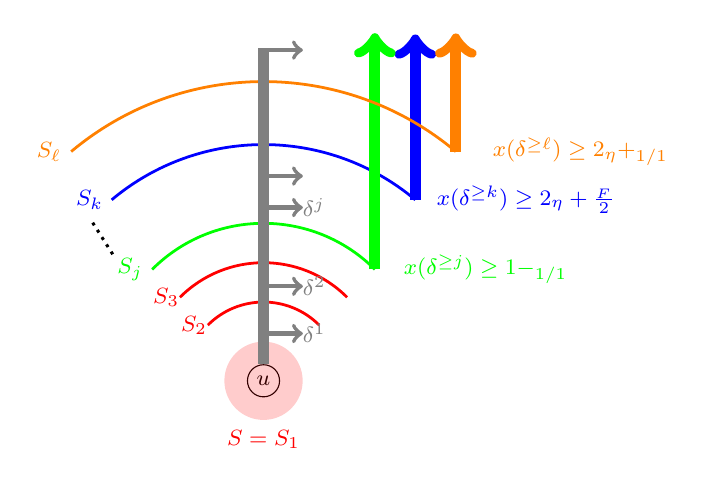
\begin{tikzpicture}
	\node [inner sep=2,draw,circle] at (0,0) (u) {\footnotesize$u$};
	\node [fill=red,opacity=0.2,circle,inner sep=10] (0,0)   () {};
	\node [color=red] at (-0,-0.75) () {\footnotesize $S=S_1$};
	\draw [line width=1pt,color=red] (45:1) arc (45:135:1) (45:1.5) arc (45:135:1.5);
	\draw [line width=1pt,color=blue] (50:3) arc (50:130:3);
	\draw [line width=4pt,color=blue,->] (50:3) -- +(0,2.1);
	\draw [line width=4pt,color=green,->] (45:2) -- +(0,3);
	\draw [line width=1pt,color=orange] (50:3.8) arc (50:130:3.8);
	\draw [line width=4pt,color=orange,->] (50:3.8) -- +(0,1.5);
	\node [xshift=45,color=orange] at (50:3.8) () {\footnotesize$x(\delta^{\geq \ell})\geq 2\eps_\eta +\eps_{1/1}$};
	\node [color=green,xshift=-8] at (135:2) () {\footnotesize$S_j$};
	\node [color=blue,xshift=-8] at (130:3) () {\footnotesize$S_k$};
	\node [color=orange,xshift=-8] at (130:3.8) () {\footnotesize$S_\ell$};
	\node [color=blue,xshift=40] at (50:3) () {\footnotesize $x(\delta^{\geq k})\geq 2\eps_\eta + \frac{\eps_F}{2}$};
	\node [color=green,xshift=40] at (45:2) () {\footnotesize $x(\delta^{\geq j})\geq 1-\eps_{1/1}$};
	\draw [color=gray,line width=1.5pt,->] (0,.6) -- node [right=3] {\footnotesize $\delta^1$} +(0.5,0);
	%\draw [color=gray,line width=1.5pt,->] (0,1.5) -- node [right=3] {\footnotesize$\delta^j$} +(0.5,0);
	\draw [color=gray,line width=1.5pt,->]  (0,1.2) -- node [right=3] {\footnotesize $\delta^2$} +(0.5,0); 
	\draw [color=gray,line width=1.5pt,->] (0,4.2) -- +(0.5,0);
	\draw [color=gray,line width=1.5pt,->]  (0,2.2) -- node [right=3] {\footnotesize$\delta^j$} +(0.5,0);
	\draw [color=gray,line width=1.5pt,->]  (0,2.6) -- +(0.5,0);
	\draw [color=green,line width=1pt]  (45:2) arc (45:135:2);
	\draw [color=gray,line width=4pt] (u) -- +(0,4.23);
	\draw [dotted,line width=1.1pt] (140:2.5) -- (137:3);
	\node [color=red,xshift=-5] at (135:1) () {\footnotesize $S_2$};
	\node [color=red,xshift=-5] at (135:1.5) () {\footnotesize $S_3$};
\end{tikzpicture}	
\end{figure}

 First, let
\begin{align*}
j&=\max\{i:x(\delta^{\ge i}) \ge  1- \eps_{1/1}\}\\
k&=\max\{i:x(\delta^{\ge i}) \ge 2\eps_{\eta} + \eps_F/2\},\\
\ell &=\max\{i:x(\delta^{\ge i}) \ge  2\eps_\eta +\eps_{1/1}\}
\end{align*}
Just note $j\leq k\leq \ell$.
Note that levels $\ell$ and $k$  exist since $x(\delta^\uparrow (u)) \ge \eps_F$, whereas level $j$ may not exist (if $x(\delta^\uparrow (u)) <  1 - \eps_{1/1}$). We consider three cases:

\paragraph{Case 1: $ x(\delta^\uparrow (u)) \ge 1- \eps_{1/1}$:}
Then $j$ exists and $S_j$ has a valid $A,B,C$ degree partitioning (\cref{def:abcdegpartitioning}) where $A = \delta(v) \cap \delta (S_j)$ such that either $u=v$ or $v$ is a descendant of $u$ in $\cH$. Note that, $x(\delta(u) \cap \delta(S_j)) \ge 1-\eps_{1/1}$, and by \cref{def:abcdegpartitioning}, $B \cap \delta(u) = \emptyset$. In addition, in this case, $x(\delta^\uparrow(u))$ is not $\eps_F$ fractional (see \cref{lem:matching}), so $\hyperlink{tar:Fu}{F_u}=1$. 
\begin{description}
\item [Case 1a:  $x(\delta^{j}) \ge 3/4$.]
If $\delta^j$ are bottom edges then \eqref{eq:toptopgoalbottom} holds. %since $\eps_{1/1}/5 \leq 0.001$ and $x(\delta^\uparrow(u))\le 1 + \eps_\eta$.
So, suppose that $\delta^j$ is a set of top edges.  
By \cref{lem:Ais211good}, at most $1/2+4\eps_{1/2}$ fraction of edges in $A\cap \delta^j$ are good but not 2-1-1 good (w.r.t., $u$). 
So, the rest of the edges in $A\cap\delta^j$ are either bad or 2-1-1 good. Since 
$$x(A\cap\delta^j)\geq 3/4-x(C)\ge  3/4-2\eps_{1/1}-\eps_\eta,$$
$\delta^j$ either has a mass  of $\frac12(1/4 - 2 \eps_{1/1} - \eps_\eta- 4 \eps_{1/2} ) > 1/8 - 3 \eps_{1/2}$ of  bad edges or of 2-1-1 good edges.\footnote{We are using the fact that $\eps_{1/1} =\eps_{1/2}/12 $ and that $\eps_\eta$ is tiny by comparison to these.}
The former case implies that \eqref{eq:toptopgoalbottom} holds. In  the latter case, by \cref{claim:211} for any 2-1-1 good edge $g\in \delta^j$ with $g\in\bbf=(u',v')$ we have  $\P{\delta(u)_T\text{ odd} | \cR_{\bbf,u'}} \leq 2\eps_\eta + \eps_{1/1}$; so  \eqref{eq:toptopgoalgoodtop}  holds for $D$ defined as the set of 2-1-1 good edges in $\delta^j$.

% of 2-1-1 good edges (w.r.t., $S_{j}$).
%Let $A,B,C$ be the degree partition of $\delta(S_j)$
%To see this, if $A$ does not contain two half edges, then there must be at least a mass of $\frac{1}{4} - \eps_{1/1} - \eps_{1/2}$ of non-1/2 edges. By \cref{lem:x_e<=1/2-eps1} and \cref{lem:x_e>=1/2+eps_1/2}, these are 2-1-1 good with respect to $S_j$.%, and this will be sufficient. 
% Otherwise, there are two good half edges $e,f$ in $\delta^j$. Then,  by \cref{lem:one-of-two-211}, one of $e,f$ is 2-1-1 good (w.r.t., $S_j$). 
%Now, if we get a mass of $1/4-\eps_{1/1}-\eps_{1/2}$ 2-1-1 good edges. Then, by \cref{claim:211}  %to the mass of at least $1/4-\eps_{1/1}-\eps_{1/2}$ of 2-1-1 good edges for $S_j$, we get 
%\begin{align*}
%\sum_{\substack{g\in \bbf=(u',v') \text{ good top},\\  g\in \delta ^\uparrow (u)}} \frac{1}{2} x_g  (\P{\delta(u)_T\text{ odd}|\cR_{\bbf,u'}} + \P{\delta(u)_T\text{ odd} | \cR_{\bbf,v'}})\\
%\le  (1/4 -\eps_{1/1}) (\frac{1}{2} + 2\eps_\eta + \eps_{1/1}) +  x(\delta^\uparrow (u)) - (1/4 -\eps_{1/1}).$$
\item [Case 1b: $x(\delta^{j}) < 3/4$.] 
If $x(\delta^\uparrow_\beta(u))\geq 0.003$, then  \eqref{eq:toptopgoalbottom} holds. % where we use the fact that $F_u = 1$.
Otherwise, we apply \cref{claim:top} with $\eps = \eps_{1/1}$ to all good top edge bundles $\bbf \in D=\delta^{\ge j +1} \smallsetminus \delta^{\ge \ell+1}$ and we get that 
$$\frac12(\P{\delta(u)_T\text{ odd}|\cR_{\bbf,u'}} + \P{\delta(u)_T\text{ odd} | \cR_{\bbf,v'}})\leq 1- \eps_{1/1}+\eps_{1/1}^2.$$
%Note that combined with any bottom edges (whose bound is only better), these edges have total fractional value at least 
Since $x(D)\geq 1-\eps_{1/1} - 3/4  - 2 \eps_\eta -\eps_{1/1}-0.003>  0.24 $,  \eqref{eq:toptopgoalgoodtop} holds. 
\end{description}
%\begin{align*}
%\sum_{f \in \delta^\uparrow (u)} \E{R_f} 
%\P{\delta (u)\text{ odd} | f\text{ red}} & \le p\tau ((1/4 - 2\eps_{1/1} - 2 \eps_\eta) (1- \eps_{1/1}) +  x(\delta^\uparrow (u)) - (1/4 -2\eps_{1/1} - 2 \eps_\eta))\\
%& < p\tau \cdot x(\delta^\uparrow (u)) \left(1- \frac{\eps_{1/1}}{5}\right),
%\end{align*}

%Using $\eps_{1/1} + \eps_\eta \le 1/40$.



\paragraph{Case 2: $ 1-\eps_F < x(\delta^\uparrow (u)) < 1- \eps_{1/1}$. } Again we have $\hyperlink{tar:Fu}{F_u}=1$.
%Then for all top edges in $\delta^\uparrow (u) \smallsetminus \delta^{\ge \ell+1} $,  \cref{claim:top} applies with $\eps = \eps_{1/1}$. 
So we can either show that $x(\delta^\uparrow_\beta(u))\geq 0.003$ or take $D$ to be the top edges in  $\delta^\uparrow (u) \smallsetminus \delta^{\ge \ell+1} $ and use \cref{claim:top} with $\eps = \eps_{1/1}$. This will enable us  to show that \eqref{eq:toptopgoalgoodtop} holds as in 
 the previous case.
%(and again, the bound for bottom edges is only better).
%Therefore, 
%\begin{align*}\sum_{f \in \delta^\uparrow (u)} \E{R_f} 
%\P{\delta (u)\text{ odd} | f\text{ red}}  &\le p\tau ( (x(\delta^\uparrow (u)) - \eps_{1/1}-2 \eps_\eta) (1-\eps_{1/1}) + \eps_{1/1} +2 \eps_{\eta}) \\
%&< p\tau \cdot x(\delta^\uparrow (u))\left(1- \frac{\eps_{1/1}}{2}\right),
%\end{align*}
%since $x_{\delta^\uparrow (u)}\ge \eps_F$, and using $2(\eps_{1/1} + 2 \eps_\eta) < \eps_F$.
%In this case, $\hyperlink{tar:Fu}{F_u}=1$ and the lemma follows.


\paragraph{Case 3: $ \eps_F < x(\delta^\uparrow (u)) < 1- \eps_F$: }
In this case $\hyperlink{tar:Fu}{F_u}=1-\eps_B$.
%\Nathan{Seeing if this approach is cleaner:}
%In this case, there is an independent probability that $u$ is even regardless of the events above $u$. Condition on any top edge $f \in \delta^\uparrow(u)$ being reduced; then, the marginals in $E(S)$ may only increase. Therefore, $\P{S \text{ is a tree} \mid f \text{ reduced}} \ge 1-\eps_\eta/2$.    
%\Nathan{Old approach:}
If at least  $4/5$ of the edges in $ \delta^\uparrow(u)$ are bottom edges, then we are done by \eqref{eq:toptopgoalbottom}.
%, using that $\frac23 \cdot 0.0035 \ge (\frac{\eps_{1/1}}{5} + 21\eps_{1/2})$ and that $\eps_{1/2}\leq 0.0001$ and $\eps_{1/1}\leq \eps_{1/2}/12$.} 
%\Nathan{It seems this means we have to make $\eps_{1/2}$ smaller} 

Otherwise, let $u'=\p(u)$. For any top edge $e\in\delta^\uparrow(u)$ where $e\in\bbf=(u'',v'')$ we have
$$ \P{\delta(u)_T\text{ odd} | \cR_{\bbf,u''}} \leq \P{u'\text{ tree}|\cR_{\bbf,u''}} \P{\delta(u)_T\text{ odd} | u'\text{ tree},\cR_{\bbf,u''}} + \P{u'\text{ not tree}| \cR_{\bbf,u''}}
%\PP{\nu}{\delta(u)_T\text{ odd} |} 
$$
Using that $u'\subseteq u''$ is a tree under $|\cR_{\bbf,u''}$ with probability at least $1-\eps_\eta/2$, and applying \cref{claim:top} (to $u$ and $u'$) with $\eps = \eps_F$ 
we have $\P{\delta(u)_T\text{ odd}|u'\text{ tree}, \cR_{\bbf,u''}}\leq 1-\eps_F+\eps_F^2$ we get
$$\P{\delta(u)_T\text{ odd} | \cR_{\bbf,u''}} \leq 1-\eps_F+\eps_F^2 + \eps_\eta/2.$$
%where $\nu=\nu_{u''}\times\nu_{G/u''}$ is the condition measure that $u'$ is a tree. 
%\cref{claim:top} applies with $\eps = \eps_F$ and $u'=S$ for all top edges in $\delta^\uparrow (u)$. 
Now, let $D$ be all top edges in $\delta^\uparrow(u)$. Then, we apply \cref{eq:toptopgoalgoodtop} to this set of mass at least $x(\delta^\uparrow(u))/5$, and we are done, using that $(\eps_F-2\eps_F^2)/5 \ge (\frac{\eps_{1/1}}{5} + \eps_B)$ which holds for $\eps_F\geq 1/10$, $\eps_B=21\eps_{1/2}$, and $\eps_{1/2}\leq 0.0002$.
\end{proof}

\begin{claim}
\label{claim:211}
For $u\in\cH$ and a top edge $e \in \bbf=(u',v')$ for some $u'\in\cH$ that is an ancestor of $u$, if
 $x(\delta  (u) \cap \delta(u')) \ge 1-\eps_{1/1}$ and $\bbf$ is 2-1-1 good, then 
	$$\P{\delta (u)_T\text{ odd} | \cR_{\bbf,u'}} \le 2\eps_\eta + \eps_{1/1}.$$
\end{claim}
\begin{proof}
Let $A,B,C$ be the \hyperlink{tar:degreepartition}{degree partitioning} of $\delta(u')$.
By the assumption of the claim, without loss of generality, assume $A\subseteq \delta(u)\cap\delta(u')$. Furthermore, by definition, $B \cap \delta(u) = \emptyset$. %or  $x(D\cap B) \ge 1-\eps_{1/1}$. 
This means that if $\cR_{\bbf,u'}=1$ then  $u'$ is a tree and $A_T = 1= (\delta  (u) \cap \delta(u'))_T$ (also using $C_T=0$ and $B \cap \delta(u) = \emptyset$). 
Therefore,
	$$\P{\delta (u)_T\text{ odd} | \cR_{\bbf,u'}} = \P{(\delta (u)\smallsetminus \delta(u'))_T \text{ even} |  \cR_{\bbf,u'}}.$$
To upper bound the RHS first observe that
$$\E{(\delta (u)\smallsetminus \delta(u'))_T| \cR_{\bbf,u'}} \leq \eps_\eta/2 + x(\delta (u)\smallsetminus \delta(u')) \leq \eps_\eta/2 + x(\delta(u)) - x(A) < 1+2\eps_\eta+\eps_{1/1}. $$
Under the conditional measure $|\cR_{\bbf,u'}$,  $u'$ is a tree ,  so $u$ must be connected inside $u'$, i.e.,  $(\delta (u)\smallsetminus \delta(u'))_T\geq 1$ with probability 1.  Therefore, 
$$\P{(\delta (u)\smallsetminus \delta(u'))_T \text{ even} |  \cR_{\bbf,u'}} \leq \P{(\delta (u)\smallsetminus \delta(u'))_T-1 \neq 0 |  \cR_{\bbf,u'}} \leq 2\eps_{\eta}+\eps_{1/1}$$
as desired.
\end{proof}

%\Nathan{Should check to see if this next lemma is stated as everyone would like}
\begin{claim}
\label{claim:top}
For $u,u'\in \cH$ such that $u'$ is an ancestor of $u$. Let $\nu=\nu_{u'}\times\nu_{G/u'}$ be the measure resulting from conditioning $u'$ to be a tree. %$e\in \bbf=(u',v')$ be a good top edge for some $u'\in\cH$ that is ancestor of $u$, if 
if $x(\delta (u) \cap \delta(u')) \in [ \eps, 1 -\eps]$, then
	\begin{equation}
	\label{eq:uandSprime}
	 \PP{\nu}{\delta (u)\text{ odd} |  (\delta(u)\cap \delta(u'))_T} \leq 1-\eps+\max\{2\eps_\eta,\eps^2\}.
	 %\P{\delta (u)\text{ odd} |\cR_{\bbf,v'}}  \le 1-\eps+\min\{2\eps_\eta,\eps^2\}.
	\end{equation}
	In other words, for any integer $k \ge 0$, we have $\PP{\nu}{\delta (u)\text{ odd} |  (\delta(u)\cap \delta(u'))_T = k} \le 1-\eps+\max\{2\eps_\eta,\eps^2\}$. 
%	where $\cal{E}$ is any event on $E(G/u')$. 
\end{claim}
\begin{proof}
%First notice conditioned on $\cR_{\bbf,u'}$
Let $D=\delta(u)\smallsetminus \delta(u')$. By assumption, $u'$ is a tree, so $D_T\geq 1$ with probability 1. Therefore, since we have no control over the parity of $(\delta(u)\cap\delta(u'))_T$
\begin{align*}
	\PP{\nu}{\delta (u)_T\text{ even} |(\delta(u)\cap\delta(u'))_T} \geq \min\{\P{D_T-1\text{ odd}|u'\text{ tree}}, \P{D_T-1=0|u'\text{ tree}}\}
\end{align*}
where we removed the conditioning by taking the worst case over $(\delta(u) \cap \delta(u'))_T$ even, $(\delta(u) \cap \delta(u'))_T$ odd. First, observe by the assumption of the claim and that $x(\delta^\uparrow(u))\leq 2+\eps_\eta$ we have
$$\E{D_T-1 | u'\text{ tree}} \in [\eps, 1 - \eps+2\eps_\eta].$$
Furthermore, since we have a SR distribution on $G[u']$, $D_T-1$ is a \hyperlink{tar:BS}{Bernoulli sum} random variable.
Therefore, 
$$\P{D_T-1=0|u'\text{ tree}}\geq \eps-2\eps_\eta$$ 
and by \cref{cor:bernoullisumeven} 
$$\P{D_T-1\text{ odd}|u'\text{ tree}} \geq 1-1/2(1+e^{-2\eps})\geq \eps-\eps^2$$
as desired. %A similar argument lower bounds $\P{\delta (u)\text{ odd} |\cR_{\bbf,v'}}$. 
%
%
%The precondition of \eqref{eq:uandSprime} and the fact that $x(\delta (u)) \in [2, 2 + \eps_\eta]$ imply that 
%$x(\delta  (u) \smallsetminus \delta(S')) \in [1 +\eps, ~2 - \eps - \eps_\eta].$
%Since conditioned on $f$ reduced, $S'$ is a tree, after conditioning, 
%$x(\delta  (u) \smallsetminus \delta(S'))$ can increase by up to $\eps_\eta$. Therefore,
%Then regardless of the parity of $U=\delta  (u) \cap \delta(S')$ after reduction, $\delta (u)$ is even with probability at least $\eps$. 
%
%Now, we compute $$\min \{\P{BS(q) \text{ even}}, \P{BS(q) \text{ odd}}\} $$. 
\end{proof}


\begin{lemma}\label{lem:xdeltau<=epsF}
Let $S\in\cH$ be a degree cut and $\bbe=(u,v)$ a good edge bundle with $\p(\bbe)=S$. If $x(\delta ^\uparrow(u)) < \eps_F$, $\eps_{1/2}\leq 0.0002$, $\eps_{1/1}\leq \eps_{1/2}/10$, then, 
$$\E{I_{\bbe,u}}+ \E{I_{\bbe,v}} \le p\tau x_\bbe \left(1 -\frac{\eps_{1/1}}{6}\right)$$ 
\end{lemma}
\begin{proof}
First notice, by \cref{lem:bottompaymentprob} for any bottom edge $g\in\delta^\uparrow(u)$ with $\p(g)=S'$, we have
$$\P{\delta(u)_T\text{ odd} | \cR_{S'}} = \P{\delta(u)_T\text{ odd} | \cE_{S'}} \leq 0.5678,$$
using $0.5678\beta \leq \tau$ and $F_u = 1$ (as $x(\delta^\uparrow(u)) \le \eps_F$) we can write,
\begin{align}\label{eq:Ieu3exp}
\E{I_{\bbe,u}} \leq	\sum_{h \in \delta ^\uparrow (u)} x_h p \tau \hyperlink{tar:Fu}{F_u}\cdot \frac{ m_{\bbe,u}}{ Z_u x (\delta ^\uparrow (u))}.
\end{align}
Secondly, if $x(\delta^\uparrow(v))\geq \eps_F$,  applying  \eqref{eq:topred} and \eqref{eq:Dec-eu} to $I_{\bbe,v}$ and using $Z_v \ge 1$ we get %and $B_u=1$ also using $B_u = Z_u = 1$ (by \cref{lem:three-nodes-good}) to show that
\begin{align}\label{eq:Ievexp3}
\E{I_{\bbe,v}} &\le \frac{m_{\bbe,v}}{\sum_{\bbf\in\delta^\rightarrow(v)} m_{\bbf,v}}
p\tau(1-\frac{\eps_{1/1}}{5})x(\delta^\uparrow(v)) \hyperlink{tar:Fu}{F_v} = m_{\bbe,v}p\tau\left(1-\frac{\eps_{1/1}}{5}\right)\hyperlink{tar:Fu}{F_v}
\end{align}
\textbf{Case 1: $|\cA(S)|=3$, where $\cA(S)=\{u,v,w\}$.} Let $\bbf = (u,w)$,  $\bbg = (v,w)$ (and of course $\bbe = (u,v)$). We will use the following facts below:  
%\begin{minipage}[c]{6cm}
\begin{figure}[htb]%{0.5\linewidth}
\centering	
	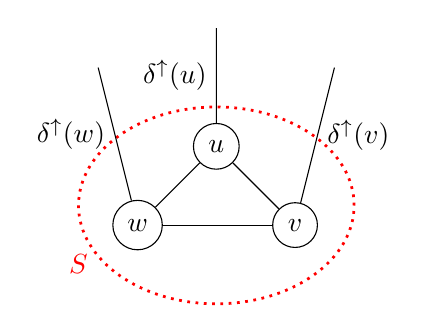
\begin{tikzpicture}
		\node[draw,circle] at (0,0) (u) {$u$};
		\node[draw,circle] at (1,-1) (v) {$v$} edge node [right] {$\bbe$} (u);
		\node[draw,circle] at (-1,-1) (w) {$w$} edge node [left] {$\bbf$} (u) edge node [below] {$\bbg$} (v);
		\draw [dotted,color=red,line width=1pt] (0,-0.75) ellipse (1.75 and 1.25);
		\draw (u) -- node [left] {$\delta^\uparrow(u)$} +(0,1.5)  
		(w) -- node [left] {$\delta^\uparrow(w)$} +(-0.5,2)
		(v) -- node [right] {$\delta^\uparrow(v)$} +(0.5,2);
		\node [color=red] at (-1.75,-1.5) (){$S$};
	\end{tikzpicture}
	%\captionof{figure}{Setting of \cref{lem:xdeltau<=epsF}.}
\end{figure}
%$x(\delta (u)) \ge 2$ and $x(\delta^\uparrow(u))\leq \eps_F$ we have 
\begin{align*}
&x_\bbe + x_\bbf \ge 2 - \eps_F \tag{$x(\delta (u)) \ge 2$ and $x(\delta^\uparrow(u))\leq \eps_F$}\\
&x(\delta ^\uparrow (v)) + x(\delta ^\uparrow (w)) \ge 2- \eps_F \tag{$x(\delta (S))\geq 2$}\\
&x_\bbf, x(\delta^\uparrow(w))\leq 1+\eps_\eta,\tag{\cref{lem:shared-edges}}
\end{align*}
so we have, 
\begin{equation}\label{eq:edeltupvlarge}x_\bbe, x(\delta ^\uparrow (v)) \ge 1- \eps_F - \eps_\eta. 	
\end{equation}


Now we bound $\E{ I_{\bbe,u}} + \E{ I_{\bbe,v}}$. By \cref{eq:Ieu3exp} and \cref{eq:Ievexp3} (which we may apply to $\E{I_{\bbe,v}}$ since $x(\delta^\uparrow(v))\geq \eps_F$),
\begin{align}
\E{I_{\bbe,u}}+\E{I_{\bbe,v}}&\leq \sum_{h \in \delta ^\uparrow (u)} x_h p \tau \hyperlink{tar:Fu}{F_u}\cdot \frac{ m_{\bbe,u}}{ Z_u x (\delta ^\uparrow (u))} +p\tau\left(1-\frac{\eps_{1/1}}{5}\right)\hyperlink{tar:Fu}{F_v} m_{\bbe,v}
\notag\\
&= p\tau \hyperlink{tar:Fu}{F_u} m_{\bbe,u}
+p\tau\left(1-\frac{\eps_{1/1}}{5}\right)\hyperlink{tar:Fu}{F_v} m_{\bbe,v} \tag{$Z_u=1$ as $|\cA(S)|=3$}\\
%\sum_{h \in \delta ^\uparrow (v)} x_h p r^*  B_v\cdot \frac{ m_{e,v}}{ x (\delta ^\uparrow (v))}\\
& = p\tau (\hyperlink{tar:Fu}{F_u}m_{\bbe,u}+\hyperlink{tar:Fu}{F_v} m_{\bbe,v}) - \frac{\eps_{1/1}}{5}p\tau \hyperlink{tar:Fu}{F_v}m_{\bbe,v} \notag\\
& \leq p\tau (1+2\eps_\eta)x_{\bbe} - \frac{\eps_{1/1}}{5}p\tau \hyperlink{tar:Fu}{F_v}m_{\bbe,v}\label{IeuIevS3}
%& \le p r^* (  B_u m_{e,u} +  \hyperlink{tar:Fu}{F_v} m_{e,v}) + p (\tau - r^*) m_{e,u}\\
%&\le  pr^* (1 + \alpha) x_e + p \tau \frac{\eps_{1/1}\eps_F(1+\alpha)}{5}\\
%&\le p \tau x_e ((1+ 2\eps_{\eta})\left((1- \frac{\eps_{1/1}}{5}) + \frac{\eps_{1/1}\eps_F}{5x_e})\right)\\
%&<p \tau x_e \left(1- \frac{\eps_{1/1}}{6}\right),
\end{align}
where the final inequality follows from \eqref{eq:uvbadematch}.
To complete the proof, we lower bound $m_{\bbe,v}$.
% Furthermore, by \cref{lem:shared-edges}  $$, it follows that $$. 

Using \eqref{eq:matchedamount} for $v$ and $w$, we can write,
\begin{align*}
x(\delta^\uparrow(v))+x(\delta^\uparrow(w)) &= m_{\bbe,v} + m_{\bbg,v} + m_{\bbf,w}+m_{\bbg,w}\\ &\leq m_{\bbe,v} +    \frac{(1+2\eps_\eta)}{(1-\eps_B)} (x_\bbf + x_{\bbg}) \tag{using \eqref{eq:uvbadematch}}\\
&= m_{\bbe,v} + \frac{(1+2\eps_\eta)}{(1-\eps_B)} \left(\sum_{a\in\cA(S)} \frac{x(\delta(a))}{2} - \frac{x(\delta(S))}{2} - x_\bbe\right)\\
&\leq m_{\bbe,v} +  \frac{(1+2\eps_\eta)}{(1-\eps_B)}  (2+3\eps_\eta-x_\bbe) %\tag{using \eqref{eq:edeltupvlarge}}
\end{align*}
and using the fact that $x(\delta^\uparrow(v))+x(\delta^\uparrow(w))\geq 2-\eps_F$, we get $$ m_{\bbe,v}\geq x_\bbe -\eps_F-4\eps_B  \geq (1- 1.2\eps_F)x_\bbe,$$ 
 %we get $m_{\bbe,v}\geq x_\bbe -\eps_F-6\eps_\eta\geq (1-\eps_F-2\eps_F^2)x_\bbe$.
 where the second inequality follows from  \eqref{eq:edeltupvlarge}
 and $\eps_B = 21 \eps_{1/2}$ and $\eps_\eta <\eps_{1/2}^2$ and $\eps_F\geq 1/10$.
Plugging this back into \eqref{IeuIevS3} and using $\hyperlink{tar:Fu}{F_v}\geq 1-\eps_B= 1-21\eps_{1/2}$ we get
$$ \E{I_{\bbe,u}}+\E{I_{\bbe,v}}\leq p\tau x_\bbe \left(1+2\eps_\eta - \frac{\eps_{1/1}}{5} (1-1.2\eps_F)(1-21\eps_{1/2})\right) \leq p\tau x_\bbe (1-\frac{\eps_{1/1}}{6}) $$
as desired. In the last inequality we used $\eps_F\leq 1/10$ and $\eps_{1/2}\leq  0.0002$.

{\bf Case 2: $|S|	\geq 4$.} 
In this case,  $Z_u = 2$. 
Therefore, by \cref{eq:Ieu3exp}
$$ \E{I_{\bbe,u}} \leq \sum_{e\in\delta^\uparrow(u)} x_e p\tau \hyperlink{tar:Fu}{F_u} \frac{m_{\bbe,u}}{Z_u x(\delta^\uparrow(u))} = \frac12 p\tau \hyperlink{tar:Fu}{F_u} m_{\bbe,u}.$$
If $x(\delta^\uparrow(v))<\eps_F$, we get the same inequality for $I_{\bbe,v}$. Then, 
$$\E{I_{\bbe,u}} + \E{I_{\bbe,v}} \le \frac12 p\tau (F_um_{\bbe,u} + F_vm_{\bbe,v}) \underset{\eqref{eq:uvbadematch}}{\le} \frac12 p\tau x_e(1+2\eps_\eta),$$
which is clearly sufficient for the lemma statement.

Otherwise, $x(\delta^\uparrow(v))\geq \eps_F$ in which case by \eqref{eq:Ievexp3} we get $\E{I_{\bbe,v}}\leq m_{\bbe,v} p\tau \hyperlink{tar:Fu}{F_v}(1-\eps_{1/1}/5)$. We conclude the lemma similar to the previous case.
%
%Therefore, for any $f \in \delta^\uparrow(u)$, we have 
%$$\E{f \text{ reduction}} 
%\P{\delta (u)\text{ odd} | f\text{ reduced}}
% \le x_f p \tau \frac{B_uZ_u}{2(1-\eps_B)}.
%$$
%so
%$$\sum_{f \in \delta ^\uparrow (u)}  \E{f \text{ reduction}} 
%\P{\delta (u)\text{ odd} | f\text{ reduced}} \cdot \frac{ m_{e,u}}{ x (\delta ^\uparrow (u))Z_u}\le p\tau \frac{B_u}{2 (1-\eps_B)} m_{e,u} <p r^* B_u m_{e,u}$$
%The rest of the argument follows as from \eqref{eq:DegreeCutPayment}.
\end{proof}

%Now we are ready to prove the main lemma of this section:
%\topincrease*
%\begin{proof}
	
%\end{proof}
%
%\anna{Take \begin{equation}
% \label{eq:taubeta1}
% \tau (1- \eps_{1/1}/5)  =   \beta (0.568 + \alpha_M).\end{equation}
% }


\subsection{Increase for Bottom Edges}\label{sub:polycutincrease}

The following lemma is the main result of this subsection.
\begin{lemma}[Bottom Edge Increase]\label{cor:botincrease}
If $\eps_{1/2}\leq 0.0002$, $\eps_{\eta} \leq \eps_{1/2}^2$, for any polygon cut $S\in\cH$,
$$\E{I_{S}} \le 0.99994 \beta p.$$	
\end{lemma}
\begin{proof}
For a set of edges $D \subseteq \delta(S)$ define the random variable.
\begin{align}I_{S}(D):=(1+\eps_\eta) (\max\{&r(A\cap D)\I{S\text{ not left happy}} , r(B\cap D)\I{S\text{ not right happy}}\}\nonumber \\
&\quad + r(C\cap D)\I{S\text{ not happy}}).\label{def:ISD}
\end{align}
Note that by definition $I_S(\delta(S))=I_S$ and for any two disjoint sets $D_1,D_2$, $I_S(D_1\cup D_2)\leq  I_S(D_1)+I_S(D_2)$.
Also, define $I_S^\uparrow = I_S(\delta^\uparrow(S))$ and $I_S^\rightarrow = I_S(\delta^\rightarrow(S))$.

First, we upper bound $\E{I^\uparrow_S}$.
Let $f\in\delta^\uparrow(S)$ and suppose that $f$ with $\p(f)=S'$ is a bottom edge. Say we have $f\in A^\uparrow(S)$ ($f \in B^\uparrow(S)$ is similar). 
We write,
\begin{align*}\E{I_S(f)}&= (1+\eps_\eta) \beta x_f \P{\cR_{S'}}\P{S \text{ not left happy } | \cR_{S'}}\\
& \le 0.568 x_f p\beta \le x_f p \tau 	
\end{align*}
where in the inequality we used \cref{lem:bottompayment-polyprob} and that 
$$\P{S\text{ not left happy} | \cR_S} = \P{S\text{ not left happy} | \cE_S}$$ 
since $\cR_S$ is a uniformly random subset of $\cE_S$. If $f \in C^\uparrow(S)$, we use the trivial guarantee $\E{I_S(f)}\le (1+\eps_\eta) x_f p \beta$. 

On the other hand, if  $f$ is a top edge, then we use the trivial bound
\begin{equation}\label{eq:trivialbottomupS}\E{I_S(f)} \le (1+\eps_\eta) \tau p x_f.	
\end{equation}
%\end{itemize}
Therefore, 
\begin{equation}
\label{eq:ISup}
\E{I_S^\uparrow} \le (1+\eps_\eta) \tau p x(\delta^\uparrow(S))  + (1+\eps_\eta)\eps_\eta p \beta \le (1+\eps_\eta) (0.571)\beta p x(\delta^\uparrow(S)) + 2\eps_\eta p \beta 
\end{equation}
since $x(C) \le \eps_\eta$.
%\end{equation}
%\anna{Later use that this is 
%\begin{equation}
%\label{eq:taubeta2}	
%\end{equation}
%\begin{equation}\le  \frac{x_e p\beta }{ 1-\eps_\eta}x_{\delta^\uparrow(S)}
%\frac{(0.568 + \alpha_M)}{1- \frac{\eps_{1/1}}{5}}.\end{equation}}

Now, we consider three cases: 

\textbf{Case 1:  $\hat{S}=\p(S)$ is a degree cut.}
Combining \eqref{eq:ISup} and \cref{lem:BT} below, we get
\begin{align*}\E{I_S} %&\leq (1+\eps_\eta) p\tau (x(\delta(S)) - (1/4-6\eps_{1/2}))\\
	&\leq (1+\eps_\eta) p(0.571)\beta (7/4+6\eps_{1/2}+\eps_\eta) + 2\eps_\eta p \beta \leq 0.99994\beta p
\end{align*}
using $\eps_{1/2}\leq 0.0002$ and $\eps_\eta\leq \eps_{1/2}^2$.

\textbf{Case 2: $\hat{S}=\p(S)$ is a polygon cut with ordering $u_1,\dots,u_k$ of $\cA(\hat{S})$, $S=u_1$ or $S=u_k$}
Then, by \cref{lem:leftmostISright} below, 
\begin{align*}
\E{I_S}\leq (1+\eps_\eta)\beta p (0.571x(\delta^\uparrow(S)) + 0.31) + 2\eps_\eta p \beta \leq 0.89 \beta p 
\end{align*}
where we used $x(\delta^\uparrow(S))\leq 1+\eps_\eta$.

\textbf{Case 3: $\hat{S}=\p(S)$ is a polygon cut with ordering $u_1,\dots,u_k$ of $\cA(\hat{S})$, $S\neq u_1, u_k$}
Then, by \cref{lem:middleISright} below
\begin{align*}
\E{I_S}\leq (1+\eps_\eta)\beta p (0.571x(\delta^\uparrow(S)) + 0.85) + 2\eps_\eta p \beta \leq 0.86 \beta p
\end{align*}
where we use that $x(\delta^\uparrow(S))\leq \eps_\eta$ since we have a \hyperlink{tar:hierarchy}{hierarchy}.
This concludes the proof.	
\end{proof}

%Let $S$ be a polygon cut (or a triangle cut) and $\hat{S}$ the parent cut of $S$ in the hierarchy. 
%Let $A,B,C$ be a partitioning of edges of $\delta(S)$ as given by \cref{def:abcpolygonpartitioning}. 
%Let
% $A^\uparrow,B^\uparrow$ be the edge bundles in $A,B$ respectively which are in $\delta^\uparrow(S)$, and similarly let $A^\rightarrow, B^\rightarrow$ be the edge bundles in $A\cap \delta^\rightarrow(S), B \cap \delta^\rightarrow(S)$. Note that $A = A^\uparrow \cup A^\rightarrow, B = B^\uparrow \cup B^\rightarrow$.  
%We have that $x(A), x(B), x(A^\rightarrow \cup B^\rightarrow) \in [1-\eps_{\eta}, 1+\eps_\eta]$;
%the upper bound is by \cref{lem:shared-edges} and the lower bound is by \cref{lem:rootedgesarebig}. 
%
%Also, since $S$ is a polygon cut, by \cref{thm:poly-structure} there are two atoms $a$ and $b$, where
% $a,b$ are the atoms left and right of the root atom of $S$ and $$A=x(\delta(a)\cap\delta(S)), B=x(\delta(b)\cap\delta(S))\geq 1-\eps_\eta\geq 1-\eps_{1/1}.$$ 
%
%
%Now recall  \eqref{eq:IeBottom} from the O-join construction that specifies how to set $I_e$, the amount by which a bottom edge $e$ inside $S$ increases to compensate for reductions in $y$ values on edges in $\delta(S)$. Using the notation $R_{\tilde E}:= \sum_{f \in \tilde E} R_f$ for any set of edges $\tilde E$, and the fact that
%${\min_{C\in\mathcal {C}} x(\delta ^\rightarrow(C))} \ge 1- \eps_\eta$, we will upper bound $I_e$ by $I_e ^\uparrow + I_e^\rightarrow$, where
%\begin{equation}
%\label{Ieup}	
%I_e^\uparrow := \frac{x_e}
%{1-\eps_\eta}\left(\sum_{f \in A^\uparrow \cap B^\uparrow} R_f \cdot \I{S \text{ not left happy (or right happy, as appropriate)}} + R_{C^\uparrow}\right)
%\end{equation}
%
%and
%
%
%\begin{equation}
%\label{Ieright}	
%I_e^\rightarrow:=\frac{x_e}
%{1-\eps_\eta}
%\left(
%\max (R_{A^\rightarrow}, R_{B^\rightarrow}) \cdot \I{S \text{ not happy}}+ R_{C^\rightarrow}
%\right).\end{equation}
%
%
%\subsubsection{Bounding $\E{I_e^\uparrow}$.}


%\subsubsection{Bounding $\E{I_e^\rightarrow}$.}

%Our analysis of \eqref{eq:Dec-eBTu2} differs depending on whether or not $\hat S$ is a degree cut or a polygon (or triangle) cut.

\subsubsection{Case 1: $\hat{S}$ is a degree cut}
\label{sec:BT}
\begin{lemma}
\label{lem:BT}
Let $S\in \cH$  be a polygon cut with parent $\hat S$ which is a degree cut. Then
$$	\E{I^\rightarrow_S} \le  (1+\eps_\eta)p\tau (x(\delta^\rightarrow(S))-(1/4-6\eps_{1/2})).$$
\end{lemma}
\begin{proof}
 Let $A,B,C$ be the polygon partition of $S$.
%For any (top) edge $e \in  \delta ^\rightarrow (S)$, we always have the trivial bound 
 %$$\E{f\text{ reduction}}\P{S\text{ not happy} | f\text{ reduced}} \le p\tau x_f.$$
 We will show that for a constant fraction of the edges in $\delta ^\rightarrow (S)$, we can improve over the trivial bound in \eqref{eq:trivialbottomupS}.
To this end, consider the cases given by \cref{thm:probabilistic}.

{\bf Case 1: There is a bad half edge $\bbe$ in $\delta ^\rightarrow(S)$.}
Since bad edges never decrease, no corresponding increase occurs, so by the trivial bound \cref{eq:trivialbottomupS}
% \eqref{eq:Dec-eBTu2} can be upper bounded by
$$\E{I_{S}^\rightarrow} \leq  (1+\eps_\eta) p\tau(x(\delta^\rightarrow(S))-(1/2-\eps_{1/2})) .$$
This concludes the proof.

{\bf Case 2: There is a set of  2-1-1 good edges  (w.r.t., $S$) $D\subseteq  \delta^\rightarrow (S)$, such that $x_{D} \ge 1/2 - \eps_{1/2}-\eps_\eta$.} 
For any (top) edge $e\in \bbf=(S,u)$ such that $e \in D$, %the reduction of $f$ is due to the event $A_{f,S}$ or $A_{f,w}$. 
if $\cR_{\bbf,S}$, then %(which happens with probability $p/2$), 
 $S$ is happy, that is $A_T=B_T=1, C_T=0$ by \cref{rem:poly-and-degree-partition}.
%\anna{A,B,C of the polygon partitioning}

%In this case, \eqref{eq:Dec-eBTu2} can be upper bounded by
Therefore,
\begin{align*}
\E{I_{S}(D)} &\le \sum_{e\in D: e\in \bbf=(S,u)} \frac{1+\eps_\eta}{2}\tau x_e \P{S\text{ not happy} | \cR_{\bbf,u}}\P{\cR_{\bbf,u}} \\
&\leq \frac{1+\eps_\eta}{2} p \tau x(D).
% \frac{ x_e}{1-\eps_\eta}\left(\sum_{f=(S,w)\in E'} \tau\E{A_{f,w}} + \sum_{f \in \delta^\rightarrow(S)\smallsetminus E'} p\tau\right)\\
%&\le  \frac{ x_ep\tau}{1-\eps_\eta}\left(\left[\frac{(1/2 - \eps_{1/2})}{2} +x(\delta ^\rightarrow (S)) - (1/2 - \eps_{1/2})\right].
%\right)
\end{align*}
Using the trivial inequality \cref{eq:trivialbottomupS} for edges in $\delta^\rightarrow(S)\smallsetminus D$ we get
$$ \E{I^\rightarrow_S} \leq (1+\eps_\eta) p\tau (\frac{x(D)}{2}+x(\delta^\rightarrow(S))-x(D)) \leq (1+\eps_\eta)p\tau (x(\delta^\rightarrow(S))-(1/4-\eps_{1/2}))$$
as desired. In the last inequality we used $x(D)\geq 1/2-\eps_{1/2}-\eps_\eta$.


{\bf Case 3: Cases 1 and 2 do not hold.} Therefore, by \cref{thm:probabilistic} there are least two 2-2-2 good top half edge bundles. In this case, $S$ has chosen a fixed pair of 2-2-2 good edges $\bbe= (S,v)$, $\bbf = (S,w)$ in $\delta ^\rightarrow(S)$ (as defined in \hyperlink{reduction-events}{the reduction events}) such that $x_{\bbe(B)},x_{\bbf(A)}\leq \eps_{1/2}$ and $\cR_{\bbe,S}=\cR_{\bbf,S}$ with probability 1. 
(Recall that $\bbe(A)=\bbe\cap A$.) Let $D=\bbe(A) \cup \bbf(B)$. 
%Observe that $x(D)\geq x_{\bbe}+x_{\bbf}-2\eps_{1/2}$
In this case, $\bbe$ and $\bbf$ are reduced simultaneously by $\tau$ when they are 2-2-2 happy (w.r.t., $S$), i.e., when $\cR_{\bbe,S}=\cR_{\bbf,S}=1$. In such a case we have $\delta(S)_T = \delta(v)_T = \delta(w)_T = 2$. 
%If these (simultaneous) reduction events occur, and $S$ is not happy, then $S$ increases by $$ (1+\eps_\eta)\max\{r_{\bbe}, r_{\bbf} \} \leq x_{\bbe}$$ 
Therefore,
\begin{align*}\E{I_S(D)} &\leq  (1+\eps_\eta) \E{\max\{r(A\cap D), r(B\cap D)\}} \\
&\leq (1+\eps_\eta) \frac{\tau}{2} \max\{x_{\bbe(A)},x_{\bbf(B)}\} (\P{\cR_{\bbe,S} \land \cR_{\bbf,S}} + \P{\cR_{\bbe,v}} + \P{\cR_{\bbf,w}}) \\
&\leq (1+\eps_\eta) \tau \frac{3p}{2} x(D)\left(\frac12+3\eps_{1/2}\right) = (1+\eps_\eta) \tau p x(D)\left(\frac34+4.5\eps_{1/2}\right)
\end{align*}
where we used that $1/2-2\eps_{1/2}-x(C)\leq x_{\bbe(A)},x_{\bbf(B)} \leq 1/2+\eps_{1/2}$ and that $x(C)\leq \eps_{\eta}$.
Using the trivial inequality \cref{eq:trivialbottomupS} for edges in $\delta^\rightarrow(S)\smallsetminus D$ we get
\begin{align*} \E{I^\rightarrow_S} &\leq (1+\eps_\eta) p\tau (x(D)(3/4+4.5\eps_{1/2})+x(\delta^\rightarrow(S))-x(D)) \\
&	\leq (1+\eps_\eta)p\tau (x(\delta^\rightarrow(S))-(1/4-6\eps_{1/2}))
\end{align*}
where we used $x(D)\geq 1-4\eps_{1/2}-\eps_\eta$.
%as desired. In the last inequality we used $x(D)\geq 1/2-\eps_{1/2}-\eps_\eta$.
%Thus,
%  \eqref{eq:Dec-eBTu2} can be upper bounded by
%  \begin{align*}
% 	\E{I_{e}^\rightarrow} & \le  \frac{ x_e}{1-\eps_\eta}\left(
% 	\E{A_{e_1,S}} \max(\tau x_{e_1}, \tau x_{e_2})
% + \sum_{f \in \delta^\rightarrow(S)\smallsetminus \{e_1, e_2\}} p\tau\right)\\
% &\le  \frac{x_e p\tau}{1-\eps_\eta}\left( \frac{\max (x_{e_1}, x_{e_2})}{2} + x(\delta ^\rightarrow (S)) - x_{e_1} - x_{e_2} \right)
%  \end{align*}
%since $\E{A_{e_1,S}} = p/2$.
%Combining this with \eqref{eq:Ieup}, we get
%$$\E{I_e} = \frac{x_e p\tau}{1-\eps_\eta}\left(x(\delta(S)) - 
%\frac{\min(x_{e_1}, x_{e_2})}{2}\right) \le  \frac{x_e p\tau}{1-\eps_{\eta}} \left(\frac{7}{4} + \eps_\eta +\frac{\eps_{1/2}}{2}\right).$$





%Combining this with \eqref{eq:Ieup}, we get that in this case.
%$$\E{I_e} = \frac{x_e p\tau}{1-\eps_\eta}\left(x(\delta(S)) - 
%x_{e'}\right) \le  \frac{x_e p\tau}{1-\eps_{\eta}} \left(\frac{3}{2} + \eps_\eta +\eps_{1/2}\right).$$
%
%
%%\end{enumerate}
%
%Using the analysis in this section, (\cref{sec:BT}), 	and observing that cases 1 and 2 give us the worst bounds,
%we conclude that
%\begin{align}
%\E{I_{e}} &\le \frac{p\tau}{1-\eps_\eta} \left(\frac{7}{4} +  \eps_{\eta} + \eps_{1/2}\right) \\
%&=
% \frac{p(0.568 + \alpha_M)\beta}{(1-\eps_\eta)(1-\eps_{1/1}/5)} \left(\frac{7}{4} + \eps_{1/2} 
% + \eps_{\eta}\right) \\
% &\le 0.996 \beta p.	
%\end{align}
%Where in the last step we use that $\eps_M,\eps_{1/1},\eps_{1,2} \le 0.0005$ and $\eps_\eta \le 0.0001$. 
%
%
\end{proof}



\subsubsection{Case 2: $S$ and its parent $\hat{S}$ are both polygon cuts}
\label{sec:BB}

%First, note that in this case, from \eqref{eq:taubeta2}, we have
%\begin{equation}
%\label{eq:IeupBB}
%	\E{I_e^\uparrow} \le  \frac{x_e p\beta }{ 1-\eps_\eta}x_{\delta^\uparrow(S)}
%\frac{(0.568 + \alpha_M)}{1- \frac{\eps_{1/1}}{5}}.
%\end{equation}

%Our goal now is to bound $\E{I_{e}^\rightarrow}$ when
% $\hat S$ is a polygon cut. There are two subcases here depending on which atom of $\hat S$, the polygon cut $S$ is.

%
%In this section, we compute the expected increase due to reductions in $A^\rightarrow$ and $B^\rightarrow$. Whenever the reduction rule (see \cref{sec:redRules}) for polygon $\hat S$ is satisfied, $A^\rightarrow$ and $B^\rightarrow$ are simultaneously reduced by $\beta x_{A^\rightarrow}, \beta x_{B^\rightarrow}$ respectively. 
%When this happens, if $S$ is not happy, edges inside $S$ will collectively increase by  $\max(\beta x_{A^\rightarrow}, \beta x_{B^\rightarrow})$. As discussed earlier, this is guaranteed to fix any odd cuts\footnote{that the increase of $\max(\beta x_{A^\rightarrow}, \beta x_{B^\rightarrow})$ is sufficient because any cut in $u$ has edges from at most one of $A^\rightarrow$ and $B^\rightarrow$.} that may exist inside $S$. 
In this subsection we prove two lemmas: \cref{lem:leftmostISright}, which bounds $\E{I_S^\rightarrow}$ when $S$ is the leftmost or rightmost atom of $\hat S$, and \cref{lem:middleISright}, which bounds this quantity when $S$ is not leftmost or rightmost.
\begin{lemma}\label{lem:leftmostISright}
Let $S\in\cH$ be a polygon cut with $\p(S)=\hat{S}$ also a polygon cut. Let $u_1,\dots,u_k$ be the ordering of cuts in $\cA(\hat{S})$ (as defined in \cref{def:hierarchy}). If $\eps_M\leq 0.001$, $\eps_\eta\leq \eps_M^2$, $S=u_1$ or $S=u_k$, then 
$$ \E{I_S^\rightarrow} \leq 0.31 \beta p.  $$
\end{lemma}
\begin{proof}
Let $S$  be the leftmost atom of $\hat{S}$
%, which we call $a_1$, and 
and let $A,B,C$ be the polygon partition of $\delta(S)$. First, note 
%We will use the following two lemmas.
%To complete the argument for this case, recall that 
\begin{equation}
\label{eq:Dec-eBTu2}
\E{I_S^\rightarrow} \le  (1+\eps_\eta) \left( \E{\max(r(A^\rightarrow), r(B^\rightarrow) ) \cdot \I{S\text{ not  happy}}} + \E{ r(C^\rightarrow)\I{S\text{ not  happy}} }
\right).
\end{equation}
where recall that $A^\rightarrow=A\cap \delta^\rightarrow(S)$. 
WLOG assume $x(A^\rightarrow)\geq x(B^\rightarrow)$. Then, 
%\begin{equation}
%\label{eq:recallIeup}\E{I_{e}^\rightarrow} \le  \frac{ x_e}{ 1-\eps_\eta}	 \left( \E{\max(R_{A^\rightarrow}, R_{B^\rightarrow} )  \I{\delta (S)\text{ not  happy}}} + \E{ R_{C^\rightarrow}}
%\right),
%\end{equation}
%and that $R_{A^\rightarrow} = \beta x_{A^\rightarrow} I_S$.

%By \cref{lem:uhappy} (see below) we can write
\begin{align*}
&\E{\max\{r(A^\rightarrow), r(B^\rightarrow)\}\I{S\text{ not happy}}} = 	
  \beta p x(A^\rightarrow) \cdot \P{S\text{ not happy} |\cR_{\hat{S}}}\\
 \intertext{By \cref{lem:uhappy} we have}
  x(A^\rightarrow) & \cdot \P{S\text{ not happy} |\cR_{\hat{S}}}
 	 \le x(A^\rightarrow)   \left(1-((1- x(A^\rightarrow))^2 + (x(A^\rightarrow))^2 -2\eps_M 
	- 17\eps_\eta)\right)  \\
	&\leq \left(2x(A^\rightarrow)^2-2x(A^\rightarrow)^3 +2\eps_M x(A^\rightarrow)+17\eps_\eta x(A^\rightarrow)\right)\\
	&\leq (8/27+2\eps_M+17\eps_\eta),
\end{align*}
where in the final inequality we used that the function $x\mapsto x^2(1-x)$ is maximized at $x=2/3$, and using $\eps_M\leq 0.00 1,\eps_\eta<\eps_M^2$.

Plugging this back into \eqref{eq:Dec-eBTu2}, and using $x(C) \le 
\eps_\eta$, we get
 $$\E{I_{S}^\rightarrow} \le  (1+ \eps_\eta)\beta p(\frac{8}{27}+2\eps_M+18\eps_\eta)\leq 0.31 \beta p, $$
 where the last inequality follows since $\eps_M\leq 0.001$ and $\eps_\eta <\eps_M^2$. 
% Combining this with \eqref{eq:IeupBB}, and using  , we get
% $$ \E{I_e} \le 
%  \frac{x_e p\beta }{ 1-\eps_\eta}\left( x_{\delta^\uparrow(S)}
%\frac{(0.568 + \alpha_M)}{1- \frac{\eps_{1/1}}{5}} + (\frac{8}{27}+2\eps_M+19.5\eps_\eta)\right) \le 0.87 x_e p\beta.$$
%since $x_{\delta^\uparrow(S)}\le 1 + \eps_\eta$ and $\eps_M \le 0.0005,\eps_\eta \le 1/10000$.	
\end{proof}

%\paragraph{Case 2(a): $S$ is the left or right-most atom of $\hat S$.} Without loss of generality, 


\begin{lemma} \label{lem:uhappy} 
Let $S\in\cH$ be a polygon cut with $\p(S)=\hat{S}$ also a polygon cut.  Let $u_1,\dots,u_k$ be the ordering of cuts in $\cA(\hat{S})$. If $S=u_1$, (or $S=u_k$) then
 $$ \P{S \text{ happy}| \cR_{\hat{S}}}%=\P{A_T=B_T=1,C_T=0 \mid \hat S \text{ reduced}} 
 \ge  (1- x(A^\rightarrow))^2 + (x(A^\rightarrow))^2 -2\eps_M 
	- 17\eps_\eta.$$	
\end{lemma}
\begin{proof}
Let $A,B,C, \hat{A},\hat{B},\hat{C}$ be the polygon partition of $S, \hat{S}$ respectively. Observe that since $S=u_1$, we have $\hat{A}= E(u_1,\overline{\hat{S}})=A^\uparrow\cup B^\uparrow\cup C^\uparrow$ and $\hat{B},\hat{C} \cap (A\cup B\cup C)=\emptyset$. 
Conditioned on $\cR_{\hat{S}}$, $\hat{S}$ is a tree,  and marginals of all edges in $\hat{A}$ is changed by a total variation distance at most $\eps'_M:=\eps_M+2\eps_\eta$ from $x$ (see \cref{cor:poly-reduction}) and they are independent of edges inside $\hat S$. The tree conditioning increases marginals inside by at most $\eps_\eta/2$.  Since after the changes just described
$$\E{C_T} \le x_C+ \eps_\eta + \eps'_M \le 4\eps_\eta +\eps_M,$$
it follows that $\P{C_T=0 | \cR_{\hat{S}}}\geq 1- 4\eps_\eta -\eps_M$.
So, 
\begin{equation}\label{eq:prob-110-before-nu}\P{S\text{ happy} \mid \cR_{\hat S}} \geq (1-4\eps_\eta - \eps_M)\P{A_T=B_T=1 | C_T=0, \cR_{\hat S}}.	
\end{equation}

Let $\nu$ be the conditional measure $C_T=0,~\cR_{\hat S}$. We see that
\begin{align*}
&\PP{\nu}{A_T=B_T=1} %= \P{A_T=B_T=1 | C_T=0, \hat S \text{ reduced}}\\
= \PP{\nu}{A_T^\uparrow = 1, B_T^\uparrow = 0, A_T^\rightarrow = 0, B_T^\rightarrow = 1} + \PP{\nu}{A_T^\uparrow = 0, B_T^\uparrow = 1, A_T^\rightarrow = 1, B_T^\rightarrow = 0} 
&\intertext{so using  independence of $(\delta^\uparrow(S))_T$ and $(\delta^\rightarrow(S))_T$.}
&\quad = \PP{\nu}{A_T^\uparrow = 1, B_T^\uparrow = 0}\PP{\nu}{A_T^\rightarrow = 0, B_T^\rightarrow = 1} + \PP{\nu}{A_T^\uparrow = 0, B_T^\uparrow = 1}\PP{\nu}{A_T^\rightarrow = 1, B_T^\rightarrow = 0}\\
%\end{align*}
%By \cref{lem:maxflow}, conditioned on $\cR_{\hat S}$, edges in $A^\uparrow$ and $B^\uparrow$ have their marginals preserved up to an additive error $\eps_M$. (They may also increase due to conditioning $C^\uparrow = 0$.) 
%\begin{align*}\intertext{using  independence of $(\delta^\uparrow(S))_T$ and $(\delta^\rightarrow(S))_T$.}
	&\quad \geq (x(A^\uparrow)-\eps'_M)\PP{\nu}{A_T^\rightarrow = 0, B_T^\rightarrow = 1} + (x(B^\uparrow)-\eps'_M)\PP{\nu}{A_T^\rightarrow = 1, B_T^\rightarrow = 0}.
\end{align*}
In the final inequality, we used the fact that conditioned on $\cR_{\hat S}$, $\hat A =(A^\uparrow \cup B^\uparrow \cup C^\uparrow)_T = 1$ and marginals in $A^\uparrow$ and $B^\uparrow$ are approximately preserved.
Now, we lower bound $\PP{\nu}{A^\rightarrow_T=1,B^\rightarrow_T=0}$. Let $\eps_A,\eps_B$ be such that 
$$ \EE{\nu}{A^\rightarrow_T}=\PP{\nu}{A^\rightarrow_T=1,B^\rightarrow_T=0}+\eps_A,\hspace{0.5cm} \EE{\nu}{B^\rightarrow_T}=\PP{\nu}{A^\rightarrow_T=0,B^\rightarrow_T=1}+\eps_B$$
First notice that $\PP{\nu}{A^\rightarrow_T + B^\rightarrow_T \ge 1} = 1$, and so $\PP{\nu}{A^\rightarrow_T + B^\rightarrow_T \ge 2} \le \EE{\nu}{A^\rightarrow_T + B^\rightarrow_T}-1$. So,
\begin{align*} \eps_A+\eps_B &= \EE{\nu}{A^\rightarrow_T+B^\rightarrow_T} - \PP{\nu}{A^\rightarrow_T+B^\rightarrow_T=1} = \EE{\nu}{A^\rightarrow_T+B^\rightarrow_T} - (1-\PP{\nu}{A^\rightarrow_T + B^\rightarrow_T \ge 2}) \\ &\le 2(\EE{\nu}{A^\rightarrow_T+B^\rightarrow_T}-1) \le 5\eps_\eta.
%&\leq (2+\eps_\eta +1.5\eps_\eta - (1-\eps_\eta)) - (1-4\eps_\eta) \leq 8\eps_\eta.
\end{align*}
To see the last inequality, first, by \cref{def:hierarchy}, $x(\delta^\uparrow(S)) \ge 1-\eps_\eta$. Since $x(\delta(S)) \le 2+\eps_\eta$, we get that $x(\delta^\rightarrow(S)) \le 1+2\eps_\eta$. Therefore, $$\EE{\nu}{A^\rightarrow_T+B^\rightarrow_T} \le \E{\delta^\rightarrow(S) \mid \cR_{\hat{S}}} \le x(\delta^\rightarrow(S)) + \eps_\eta/2 \le 1+2.5\eps_\eta.$$
%where in the inequality we used $x(\delta(S))\leq 2+ \eps_\eta$,
%(by \cref{lem:smallatoms}), 

%where we use that conditioning $\hat{S}$ to be a tree and $C$ to 0 increases marginals by at most $1.5\eps_\eta$, that $x(\delta^\uparrow(S))\geq 1-\eps_\eta$ (by \cref{lem:rootedgesarebig}) and \cref{lem:ApBright=1}.
Therefore, 
\begin{align*}
\PP{\nu}{A_T=B_T=1}	&\geq (x(A^\uparrow)-\eps'_M) (\EE{\nu}{B^\rightarrow_T}-\eps_B) + (x(B^\uparrow)-\eps'_M) (\EE{\nu}{A^\rightarrow_T}-\eps_A)\\
&\geq (x(A^\uparrow)-\eps'_M)  (x(B^\rightarrow)-5\eps_\eta) + (x(B^\uparrow)-\eps'_M)(x(A^\rightarrow)-5\eps_\eta)
\end{align*}
where the second inequality uses that the  tree conditioning and $C^\rightarrow_T=0$ can only increase the marginals of edges in $A^\rightarrow$ and $B^\rightarrow$.
Simplify the above using  $x(A^\uparrow)  +x(A^\rightarrow) \ge 1-\eps_\eta$, and similarly for $B$,  
\begin{align*}
	&\PP{\nu}{A_T=B_T=1} \\
	&\ge (1- x(A^\rightarrow) - \eps_\eta-\eps'_M) (x(B^\rightarrow)-5\eps_\eta) + (1- x(B^\rightarrow) - \eps_\eta -\eps'_M)(x(A^\rightarrow)-5\eps_\eta) \\ 
	\intertext{ and since $x(A^\rightarrow) + x(B^\rightarrow) \ge 1- 2\eps_\eta$ (because
$x(A^\uparrow) + x(B^\uparrow) \le 1+ \eps_\eta$ and $x_C \le \eps_\eta$), this is}
	&\ge (1- x(A^\rightarrow) - \eps_\eta-\eps'_M) (1 - x(A^\rightarrow)-7\eps_\eta) + (x(A^\rightarrow) - 3\eps_\eta -\eps'_M)(x(A^\rightarrow)-5\eps_\eta) \\
	&\ge   (1- x(A^\rightarrow))^2 + (x(A^\rightarrow))^2 -\eps'_M 
	- 8\eps_\eta.
	\end{align*}
Plugging this into \cref{eq:prob-110-before-nu}, we obtain 
\begin{align*}
\P{A_T=B_T=1,C_T=0 \mid \cR_{\hat S}} &\geq (1-2\eps_\eta - \eps'_M)\P{A_T=B_T=1 | C_T=0, \cR_{\hat S}} \\
& \ge (1-2\eps_\eta - \eps'_M)((1- x(A^\rightarrow))^2 + (x(A^\rightarrow))^2 -\eps'_M - 8\eps_\eta) \\
& \ge (1- x(A^\rightarrow))^2 + (x(A^\rightarrow))^2 -2\eps'_M - 10\eps_\eta,
\end{align*}
which noting $\eps'_M=\eps_M+2\eps_\eta$ completes the proof of the lemma. 
\end{proof}



%\begin{claim}\label{lem:ApBright=1}
%Let $\nu$ be the conditional measure $C_T=0, \cR_{\hat S}$. Then
%	 $$\PP{\nu}{A^\rightarrow_T +B^\rightarrow_T = 1} \ge 1-4\eps_\eta.$$ 
%\end{claim}
%\begin{proof}
%First, notice under $\nu$, $\hat S$ is a tree, and $\delta^\rightarrow(S)$ is independent of edges in $G/\hat{S}$, though $\EE{\nu}{\delta^\rightarrow(S)_T}$ may be increased by $2\eps_\eta$ due to $\cR_{\hat{S}}$, $C_T=0$, so
%$$ \EE{\nu}{\delta^\rightarrow(S)_T} \leq 2+\eps_\eta - (1-\eps_\eta) + 2\eps_\eta \leq 1+4\eps_\eta,$$
%where we used that $S=u_1$, so $x(\delta^\uparrow(S))\geq 1-\eps_\eta$.
%
%Also, since $C_T=0$, under $\nu$, we have $\delta^\rightarrow(S)_T=A^\rightarrow_T+B^\rightarrow_T$. Furthermore, since $\delta^\rightarrow(S)_T\geq 1$ with probability 1 under $\nu$,  
%$$ \PP{\nu}{A^\rightarrow_T+B^\rightarrow_T=1} = \PP{\nu}{\delta^\rightarrow(S)_T=1 } \geq 1-4\eps_\eta$$
%as desired.
% Recall that $u_1,\dots,u_k$ is the ordering of atoms in $\cA({\hat S})$ and $S=u_1$.
%Since $u_1,u_2\in\cH$, 
%$x(\delta(u_1)),x(\delta(u_2)) \le 2+\eps_\eta.$ 
%So by \cref{lem:treeconditioning},
%$$\PP{\nu}{u_1\text{ tree}}, \PP{\nu}{u_2\text{ tree}}\geq 1-\frac12\eps_\eta.$$
%On the other hand, since $\cH$ is a \hyperlink{tar:hierarchy}{hierarchy}, $x(E(\{u_1,u_2\})) \le 1-\eps_\eta$, 
%so
%$$ \PP{\nu}{u_1\cup u_2\text{ tree}}\geq 1-3\eps_\eta.$$
%The extra $\eps_\eta$ come from the fact that in the worst case $C$ is a subset of $E(u_1,u_2)$.
%
%%%Note that conditioning $\hat S$ to be a tree and $C_T=0$ can only increase marginals of $E(S), E(S')$ and this can only increase the probability that $S$ and $S'$ are trees.
%
%
%
%
%%Let $\nu$ be the conditional measure $C_T=0, ~ \hat S\text{ reduced}$.
%Next, observe that
%$$\EE{\nu}{\delta^\rightarrow(u_1)}= \EE{\nu}{\delta(u_1)- 
%\hat{A}} \le \E{\delta(u_1)- 
%\hat{A}} + \eps_\eta \le  2 + \eps_\eta - (1-\eps_\eta) + \eps_\eta =1+3\eps_\eta.$$
%The $\eps_\eta$ in the first inequality is from tree conditioning; conditioning $C_T=0$ only helps. Also recall that $\hat{A},\hat{B},\hat{C}$ is the polygon partition of $\hat{S}$, so $x(\delta^\uparrow(u_1))=x(\hat{A})\geq 1-\eps_\eta$. 
%% Last term is $E(u,u')$.
%%This combined with the fact that  $x(E(u_1,u_2))\geq 1-\eps_\eta$  implies that 
%Therefore,
%$$\EE{\nu}{\delta^\rightarrow(u_1) \smallsetminus E(u_1,u_2)} \le  1+3\eps_\eta - (1-\eps_\eta) \leq 4\eps_\eta.$$ 
%
%Finally, by a union bound, $u_1,u_2,\{u_1,u_2\}$ are all trees, and $(\delta^\rightarrow(u_1)  \smallsetminus E(u_1,u_2))_T = 0$ simultaneously with probability at least $1-8\eps_\eta$. 
%So, this implies $\delta^\rightarrow(u_1)_T = A^\rightarrow_T+B^\rightarrow_T+C^\rightarrow_T=1$ which proves the claim since $C_T=0$.
%%\Shayan{We should make this a separate lemma as we use it several times.}
%\end{proof} 
%We use this to bound the probability of the event that $S$ is not happy given that $\hat S$ is reduced.
 
 


%\vspace{0.1in}
 
 
 
 \begin{lemma}\label{lem:middleISright}
Let $S\in\cH$ be a polygon cut with $\p(S)=\hat{S}$ also a polygon cut with $u_1,\dots,u_k$ be the ordering of cuts in $\cA(\hat{S})$. If $S\neq u_1,u_k$, then 
$$ \E{I_S^\rightarrow} \leq  0.85 \beta p.$$
\end{lemma}

 
\begin{proof}
Let $S=u_i$ for some $2\leq i\leq k-1$.
 Let $A,B,C$ be the polygon partitioning of  $\delta(u_i)$ and $\hat{A},\hat{B},\hat{C}$ be the polygon partition of $\hat{S}$.
 Since $u_i$ is in the \hyperlink{tar:hierarchy}{hierarchy} $A^\uparrow\cup B^\uparrow\cup C^\uparrow\subseteq \hat{C}$.
 So, conditioned on $\cR_{\hat{S}}$, $A^\uparrow_T= B^\uparrow_T= C^\uparrow_T=0$.
 
Once again, let $\nu$ be the conditional measure $C_T=0,~ \cR_{\hat{S}}$. Similar to the previous case, we will lower-bound
%$ \P{S\text{ happy} | \cR_{\hat{S}}}.$
%Furthermore, $\E{x_{C^\rightarrow} | \hat S\text{ reduced}}\leq 2\eps_\eta$. So, we have
\begin{align}
\P{S\text{ happy} |\cR_{\hat{S}}} &\geq (1-2\eps_\eta) \P{A^\rightarrow_T=1,B^\rightarrow_T=1,| C_T=0,  \cR_{\hat{S}}}\nonumber\\
&=(1-2\eps_\eta) \PP{\nu}{A^\rightarrow_T=1 | A^\rightarrow_T+B^\rightarrow_T=2}\PP{\nu}{A^\rightarrow_T+B^\rightarrow_T=2 }
\label{eq:bbhappyGreduced}
\end{align}
where we used $\E{C^\rightarrow_T | \cR_{\hat{S}}} \leq 2\eps_\eta$ in the first inequality. 
So, it remains to lower-bound each of the two terms in the RHS. 

We start with the first one. Since $x(A)\in [1-\eps_\eta,1+\eps_\eta]$ and $x(A^\uparrow)\leq \eps_\eta$ we have
$$ \EE{\nu}{A^\rightarrow_T}\in [1-2\eps_\eta,1+3\eps_\eta]. % \leq x(A^\rightarrow)+2\eps_\eta \leq 1+3\eps_\eta
$$
%where the first inequality uses $1-\eps_\eta \leq x(A)$ and $x(A^\uparrow)\leq \eps_\eta$ by \cref{lem:rootedgesarebig}. The second and third inequalities uses that marginals of $A^\rightarrow$ increase by at most $2\eps_\eta$ due to conditioning $\hat S$ to be a tree and $(C^\rightarrow)_T=0$. Finally, the last inequality uses that $x(A^\rightarrow)\leq x(A)\leq 1+\eps_\eta$ by \cref{lem:shared-edges}.  
The same bounds hold for $\EE{\nu}{x(B^\rightarrow)}$. 

Therefore,
\begin{align*}
&\PP{\nu}{A^\rightarrow_T \ge 1}, \PP{\nu}{B^\rightarrow_T\geq 1} \geq 1-e^{-1+2\eps_\eta}
%= 1 - \PP{\nu}{A_T = 0} \ge 1 - \left(1-\frac{1-2\eps_\eta}{n}\right)^n \ge 
 \tag{\cref{lem:SR>=}} \\
&\PP{\nu}{A^\rightarrow_T\leq 1},\PP{\nu}{B^\rightarrow_T\leq 1} \geq 0.495 \tag{Markov}
\end{align*}

%and $\PP{\nu}{A_T \le 1}$ can be bounded using expectation:
%$$1+3\eps_\eta \ge \EE{\nu}{x(A)} \ge 2(1-\PP{\nu}{A_T \le 1})$$
%It follows that $\PP{\nu}{A_T \le 1} \ge 1/2-3/2\eps_\eta$. And similarly for $B_T$. 
%(This can be improved by using the fact that probability it's at least 2 is at most $1-2/e$.)

Therefore, by \cref{lem:SRA=nA} (with $\eps=0.495(1-e^{-1+2\eps_\eta})\geq 0.31$) we have
$$\PP{\nu}{A^\rightarrow_T =1 \mid A^\rightarrow_T + B^\rightarrow_T = 2} \ge 0.155.$$ 
%Using $\eps_\eta \le \frac{1}{1000}$, both quantities are at least 0.15. Therefore by \cref{lem:logconcavity},
%$$\PP{\nu}{A_T = 1 \mid A_T + B_T = 2} \ge \frac{1}{2}0.15 = 0.075$$
%Finally, since $\EE{\nu}{(A\cup B)_T} \ge 2-4 \eps_\eta$, we have $\PP{\nu}{A_T + B_T = 2} \ge \left(1-\frac{1-4\eps_\eta}{n}\right)^n \ge e^{-1+4\eps_\eta} \ge 0.37$. Therefore 
By \cref{lem:treeoneedge}, 
%an argument similar to the proof of \cref{lem:ApBright=1} %since $u_{i-1},u_i\in\cH$ and $x(E(u_{i-1},u_i))\geq 1-\eps_\eta$, 
%$$\PP{\nu}{u_i,u_{i-1},u_i\cup u_{i-1}\text{ trees}}\geq  1-4\eps_\eta.$$ 
%So, 
$\PP{\nu}{E(u_{i-1},u_i)_T=1}\geq 1-4\eps_\eta$. Similarly, $\PP{\nu}{E(u_{i},u_{i+1})_T=1}\geq 1-4\eps_\eta$. And, 
$$\PP{\nu}{\delta^\rightarrow(u_i)_T- E(u_{i-1},u_i)_T -E(u_i,u_{i+1})_T=0} \geq 1-4\eps_\eta$$
So, by a union bound all of these events happen simultaneously and we get $\PP{\nu}{\delta^\rightarrow(u_i)_T=2}\geq 1-12\eps_\eta$.
Therefore,
$$ \PP{\nu}{(A^\rightarrow)_T=(B^\rightarrow)_T=1} \geq 0.155 (1-12\eps_\eta) \ge 0.153.$$
Plugging this back into \eqref{eq:bbhappyGreduced}, we get
$$ \P{S\text{ happy} | \cR_{\hat{S}}}\geq 0.153(1-2\eps_\eta) \ge 0.152.$$
Plugging this in \eqref{eq:Dec-eBTu2}
we get
\begin{align*} \E{I_S^\rightarrow}&\leq (1+\eps_\eta)\beta p \P{S\text{ not happy}|\cR_{\hat{S}}}(\max\{x(A^\rightarrow),x(B^\rightarrow)\} + x(C^\rightarrow)) \\
	&\leq (1+\eps_\eta) \beta p (1-0.152) (1+\eps_\eta+\eps_\eta) \leq 0.85 \beta p
\end{align*}
as desired.
%Putting it all together, yields
% $$ \E{I_e} \le 
%  \frac{x_e p\beta }{ 1-\eps_\eta}\left( x(\delta^\uparrow(S))
% + \max\{x(A^\rightarrow), x(B^\rightarrow)\}\left(1-\frac{1}{50}\right) + x(C^\rightarrow)\right) \le 0.981 x_e p\beta,$$
%using $x_{\delta^\uparrow(u)},x_{C^\rightarrow} \le \eps_\eta$ and $\eps_\eta \le \frac{1}{10000}$. For simplicity we remove the conditional probability for the component $\delta^\uparrow(S)$. 

\end{proof}
%The above analysis proves the following lemma. We note that in the second case the analysis is not tight. 
%\begin{lemma}
%\label{lem:BB}
%Suppose that $S$ is a polygon with parent $\hat S$ which is also a polygon cut. Then
%$$	\E{I_{e}} \le 0.981 \beta p.$$
%\end{lemma}
%
%This lemma together with \cref{lem:BT} proves \cref{cor:botincrease}.





